\chapter{Resultados}\label{cap:resultados}

Este capítulo relata os resultados obtidos com a aplicação da coerência \textit{Wavelet}
alternativa de \citeonline{schuck2019} aos sinais espaciais de brilho reconstruídos do panorama
das imagens, conforme a metodologia descrita no \autoref{cap:metodologia}. A apresentação segue a
ordem do \textit{pipeline}: primeiro os sinais espaciais reconstruídos, depois os campos de
espectro de potência (WPS) e o perfil de potência média por padrão, em seguida os campos de
coerência (WCO), e por fim as duas leituras comparativas visadas pelo trabalho, a repetibilidade
intra-padrão e a separação inter-padrão. A inspeção dos campos é qualitativa. A
\autoref{sec:res-limite-estat} complementa essa leitura com a quantificação estatística da
repetibilidade do perfil de potência média para os quatro padrões com mais de dois ensaios.

% =========================================================
\section{Campanhas de processamento intra e inter-padrão}\label{sec:res-visao}
% =========================================================

O cálculo da coerência \textit{Wavelet} alternativa foi executado em duas campanhas
complementares sobre os ensaios elegíveis descritos na \autoref{sec:met-dados}. A campanha
intra-padrão cobriu os noventa e um pares de ensaios de um mesmo padrão, e a campanha inter-padrão
cobriu os duzentos e oitenta e sete pares de ensaios de padrões distintos. As duas campanhas
empregaram o mesmo cálculo, diferindo apenas na regra de emparelhamento dos ensaios: a campanha
intra-padrão compara dois ensaios do \textit{mesmo} padrão, para verificar se a assinatura
espectral \textit{se repete}, e a inter-padrão compara ensaios de padrões \textit{diferentes},
para verificar se a assinatura \textit{distingue} um padrão do outro.

Para cada par de ensaios, o processamento produziu os campos de espectro de potência
$\widetilde{P}_x(a)$ e $\widetilde{P}_y(a)$ de cada ensaio, o campo de espectro cruzado
$\widetilde{C}_{xy}(a)$ e o campo de coerência $\widetilde{\gamma}_{xy}(a)$, além dos perfis de
potência média $|\text{WPS}|$ por comprimento de onda. Cada par foi processado nas duas variantes
do sinal espacial descritas na \autoref{sec:met-dados}: a variante \textit{cropped}, obtida pela
média das linhas 20 a 59 do panorama, e a variante \textit{center}, obtida da linha central 40.
As figuras deste capítulo referem-se à variante \textit{cropped}, que reúne o núcleo do escoamento.

O \autoref{quad:res-ensaios} relaciona todos os ensaios processados, com o padrão rotulado, o
nível de fluxo mássico $G$ e de fluxo de calor $q$ de cada ponto operacional e o comprimento $N$ do
sinal espacial, igual à largura do panorama reconstruído em pixels. O comprimento varia de alguns
milhares a mais de vinte mil pixels, acompanhando a velocidade do escoamento: ensaios de regime
rápido percorrem a seção de visualização em menos quadros e produzem panoramas mais curtos, ao
passo que ensaios de regime mais lento produzem panoramas mais longos. Os ensaios de regime anular
ondulado concentram-se nos comprimentos mais longos, e os intermitentes (\textit{plug} e
\textit{slug}), nos mais curtos.

\begin{quadro}[htb]
  \centering
  \caption{Ensaios processados, por padrão, com o nível de fluxo mássico $G$ e de fluxo de calor
           $q$ do ponto operacional e o comprimento $N$ do sinal espacial (largura do panorama
           reconstruído, em pixels, na variante \textit{cropped}).}
  \label{quad:res-ensaios}
  \begin{tabular}{l l c c r}
    \hline
    \textbf{Ensaio} & \textbf{Padrão} & \textbf{$G$} & \textbf{$q$} & \textbf{$N$ (px)} \\
    \hline
    m03q05 & \textit{Churn} & 3 &  5 &  9586 \\
    m04q10 & \textit{Churn} & 4 & 10 &  8829 \\
    m04q20 & \textit{Churn} & 4 & 20 &  9344 \\
    m05q10 & \textit{Churn} & 5 & 10 &  7001 \\
    m05q20 & \textit{Churn} & 5 & 20 &  7391 \\
    m05q40 & \textit{Churn} & 5 & 40 &  9937 \\
    m06q10 & \textit{Churn} & 6 & 10 &  7584 \\
    m06q20 & \textit{Churn} & 6 & 20 & 10044 \\
    m07q20 & \textit{Churn} & 7 & 20 &  8255 \\
    m07q40 & \textit{Churn} & 7 & 40 & 10349 \\
    \hline
    m03q10 & Anular ondulado & 3 & 10 & 14224 \\
    m03q20 & Anular ondulado & 3 & 20 & 23079 \\
    m03q40 & Anular ondulado & 3 & 40 & 20743 \\
    m04q40 & Anular ondulado & 4 & 40 & 14960 \\
    m04q80 & Anular ondulado & 4 & 80 & 22636 \\
    m05q80 & Anular ondulado & 5 & 80 & 17524 \\
    m06q40 & Anular ondulado & 6 & 40 & 14772 \\
    m06q80 & Anular ondulado & 6 & 80 & 18665 \\
    m07q80 & Anular ondulado & 7 & 80 & 16658 \\
    \hline
    m05q01    & \textit{Plug} & 5 &  1 & 5940 \\
    m05q05\_2 & \textit{Plug} & 5 &  5 & 4510 \\
    m06q01    & \textit{Plug} & 6 &  1 & 7798 \\
    m07q05    & \textit{Plug} & 7 &  5 & 7358 \\
    \hline
    m04q01    & \textit{Slug} & 4 & 1 & 5071 \\
    m05q05\_1 & \textit{Slug} & 5 & 5 & 6323 \\
    m06q05    & \textit{Slug} & 6 & 5 & 7787 \\
    \hline
    m04q05 & \textit{Slug}--\textit{churn} & 4 &  5 & 5460 \\
    m07q10 & \textit{Slug}--\textit{churn} & 7 & 10 & 9101 \\
    \hline
  \end{tabular}
  \fonte{Elaborado pelo autor.}
\end{quadro}

% =========================================================
\section{Panoramas reconstruídos por padrão}\label{sec:res-panorama}
% =========================================================

Antes de descrever os sinais e os campos espectrais, convém observar a imagem que lhes dá origem.
O \textit{panorama} de cada ensaio é a reconstrução espacial descrita na
\autoref{sec:met-dados}: uma tira de altíssima razão de aspecto, costurada quadro a quadro, em que
o eixo horizontal corresponde à posição ao longo do percurso do escoamento no tubo e cada coluna
registra o brilho naquela posição. O sinal espacial de brilho analisado adiante é extraído
diretamente desse panorama, pela média das linhas 20 a 59 na variante \textit{cropped}. Observar o
panorama ajuda a reconhecer, de forma visual e direta, a textura característica de cada padrão
antes de reduzi-la a uma curva unidimensional.

A \autoref{fig:res-panorama-plug} e a \autoref{fig:res-panorama-slug} mostram os panoramas de
\textit{plug} e de \textit{slug}. Nos dois padrões, intermitentes, o escoamento alterna bolhas
alongadas discretas com grandes trechos de líquido entre elas, de modo que o panorama exibe
estruturas claras bem espaçadas sobre um fundo mais uniforme. A distinção entre \textit{plug} e
\textit{slug} é gradual: as bolhas do \textit{slug} são mais longas e mais frequentes do que as do
\textit{plug}. A \autoref{fig:res-panorama-churn} mostra o panorama de \textit{churn}, de aparência
densa e desorganizada, sem estruturas discretas bem definidas, refletindo o caráter agitado e
caótico desse regime. A \autoref{fig:res-panorama-annular} mostra o panorama de anular ondulado,
em que um filme contínuo recobre a parede e a interface apresenta uma ondulação fina e regular ao
longo de todo o percurso, textura visualmente mais homogênea do que a do \textit{churn}.

A comparação visual entre os quatro panoramas revela que os padrões se distinguem sobretudo pela
\textit{escala} e pela \textit{regularidade} das estruturas, e não por uma forma facilmente
descritível a olho. Os regimes intermitentes (\textit{plug} e \textit{slug}) apresentam estruturas
grandes e espaçadas; \textit{churn} apresenta estruturas pequenas e desorganizadas; e o anular
ondulado apresenta uma ondulação fina e repetitiva. Essa observação qualitativa antecipa o
resultado central do capítulo: a característica que separa os padrões é a distribuição de energia
por comprimento de onda, quantificada no espectro de potência da \autoref{sec:res-wps}, e não a
forma bruta do sinal unidimensional dela derivado.

\begin{figure}[htbp]
  \centering
  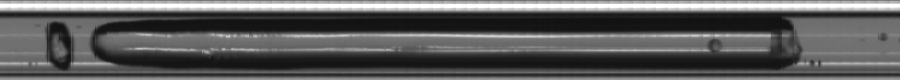
\includegraphics[width=\textwidth]{figuras/v8-panorama-plug}
  \caption{Trecho inicial do panorama espacial reconstruído de um ensaio de \textit{plug}
           (primeiras 900 colunas, de um total de 5940). O eixo horizontal corresponde à posição
           ao longo do percurso do escoamento; bolhas alongadas discretas alternam-se com trechos
           de líquido mais uniformes.}
  \label{fig:res-panorama-plug}
  \fonte{Elaborado pelo autor.}
\end{figure}

\begin{figure}[htbp]
  \centering
  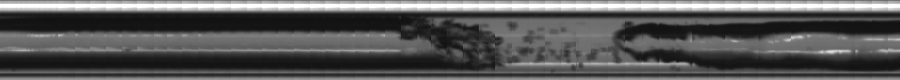
\includegraphics[width=\textwidth]{figuras/v8-panorama-slug}
  \caption{Trecho inicial do panorama espacial reconstruído de um ensaio de \textit{slug}
           (primeiras 900 colunas, de um total de 5071). As bolhas alongadas são mais longas e
           mais frequentes do que no \textit{plug}, mantido o fundo de líquido entre elas.}
  \label{fig:res-panorama-slug}
  \fonte{Elaborado pelo autor.}
\end{figure}

\begin{figure}[htbp]
  \centering
  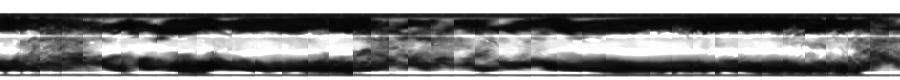
\includegraphics[width=\textwidth]{figuras/v8-panorama-churn}
  \caption{Trecho inicial do panorama espacial reconstruído de um ensaio de \textit{churn}
           (primeiras 900 colunas, de um total de 9586). A textura é densa e desorganizada, sem
           estruturas discretas bem definidas, refletindo o caráter agitado do regime.}
  \label{fig:res-panorama-churn}
  \fonte{Elaborado pelo autor.}
\end{figure}

\begin{figure}[htbp]
  \centering
  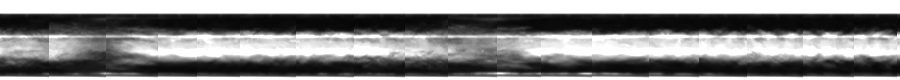
\includegraphics[width=\textwidth]{figuras/v8-panorama-annular}
  \caption{Trecho inicial do panorama espacial reconstruído de um ensaio de anular ondulado
           (primeiras 900 colunas, de um total de 23079). Um filme contínuo recobre a parede e a
           interface exibe uma ondulação fina e regular ao longo do percurso.}
  \label{fig:res-panorama-annular}
  \fonte{Elaborado pelo autor.}
\end{figure}

% =========================================================
\section{Sinais espaciais reconstruídos}\label{sec:res-sinais}
% =========================================================

Os sinais espaciais de brilho reconstruídos do panorama apresentaram-se como séries de milhares de
amostras por ensaio, com uma amostra por pixel de percurso do escoamento no tubo. Após a remoção de
tendência, da média e a normalização pelo desvio padrão, cada sinal ficou centrado em zero e com
variância unitária, expresso em unidades de desvio padrão. A \autoref{fig:res-sinais} mostra os
sinais de dois ensaios de \textit{churn}, sobrepostos no painel inferior. O brilho oscila ao longo
do eixo de percurso sem tendência residual, refletindo a passagem sucessiva das estruturas do
escoamento pela seção de visualização.

A mesma reconstrução foi obtida para os demais padrões, ilustrada nas
\autoref{fig:res-sinais-annular}, \autoref{fig:res-sinais-plug} e \autoref{fig:res-sinais-slug} para
anular ondulado, \textit{plug} e \textit{slug}, respectivamente. Os ensaios de \textit{plug} e de
\textit{slug} foram reconstruídos e analisados mesmo dispondo de poucos ensaios, quatro e três,
respectivamente, de modo que a sua inclusão tem caráter ilustrativo; essa limitação de amostragem é
retomada na discussão. Em
unidades de desvio padrão, os sinais crus dos quatro padrões têm aparência semelhante, uma oscilação
irregular em torno de zero, sem que a inspeção direta do sinal no tempo revele qual padrão o
originou. A característica que distingue os padrões não está na forma bruta do sinal, mas na
distribuição de energia por comprimento de onda, examinada no espectro de potência da
\autoref{sec:res-wps}.

\begin{figure}[htbp]
  \centering
  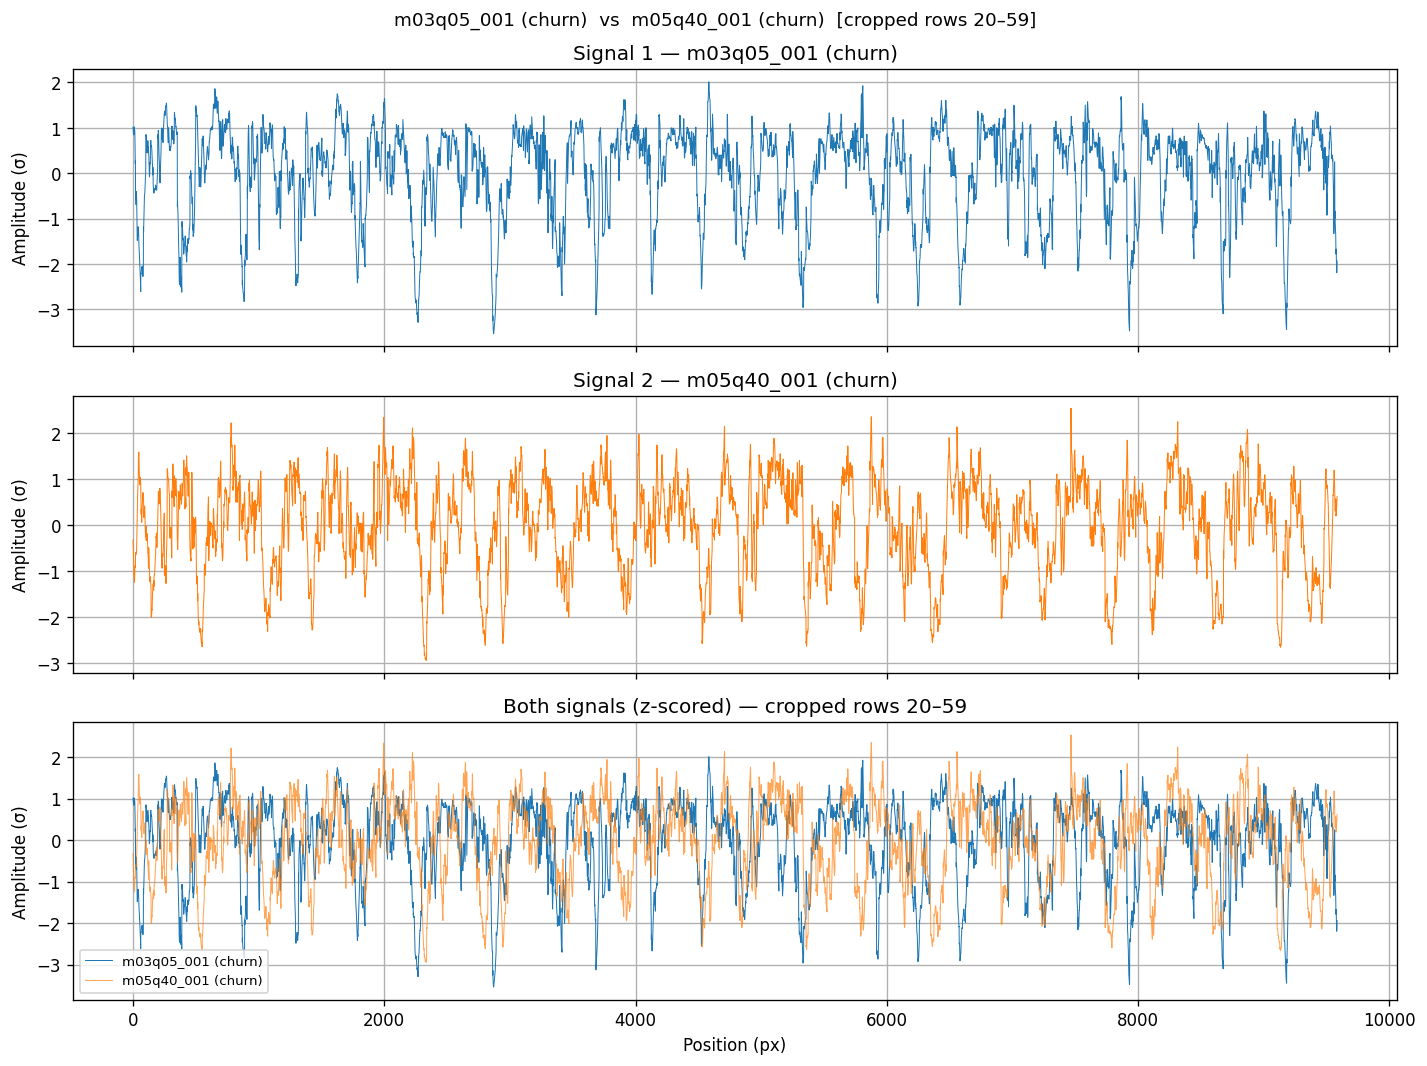
\includegraphics[width=0.92\textwidth]{figuras/v8-churn-churn-signals}
  \caption{Sinais espaciais de brilho de dois ensaios de \textit{churn}, na variante
           \textit{cropped} (média das linhas 20 a 59 do panorama), após pré-processamento.
           Painéis superior e central: cada ensaio isoladamente. Painel inferior: os dois sinais
           sobrepostos, em unidades de desvio padrão, ao longo da posição em pixels.}
  \label{fig:res-sinais}
  \fonte{Elaborado pelo autor.}
\end{figure}

\begin{figure}[htbp]
  \centering
  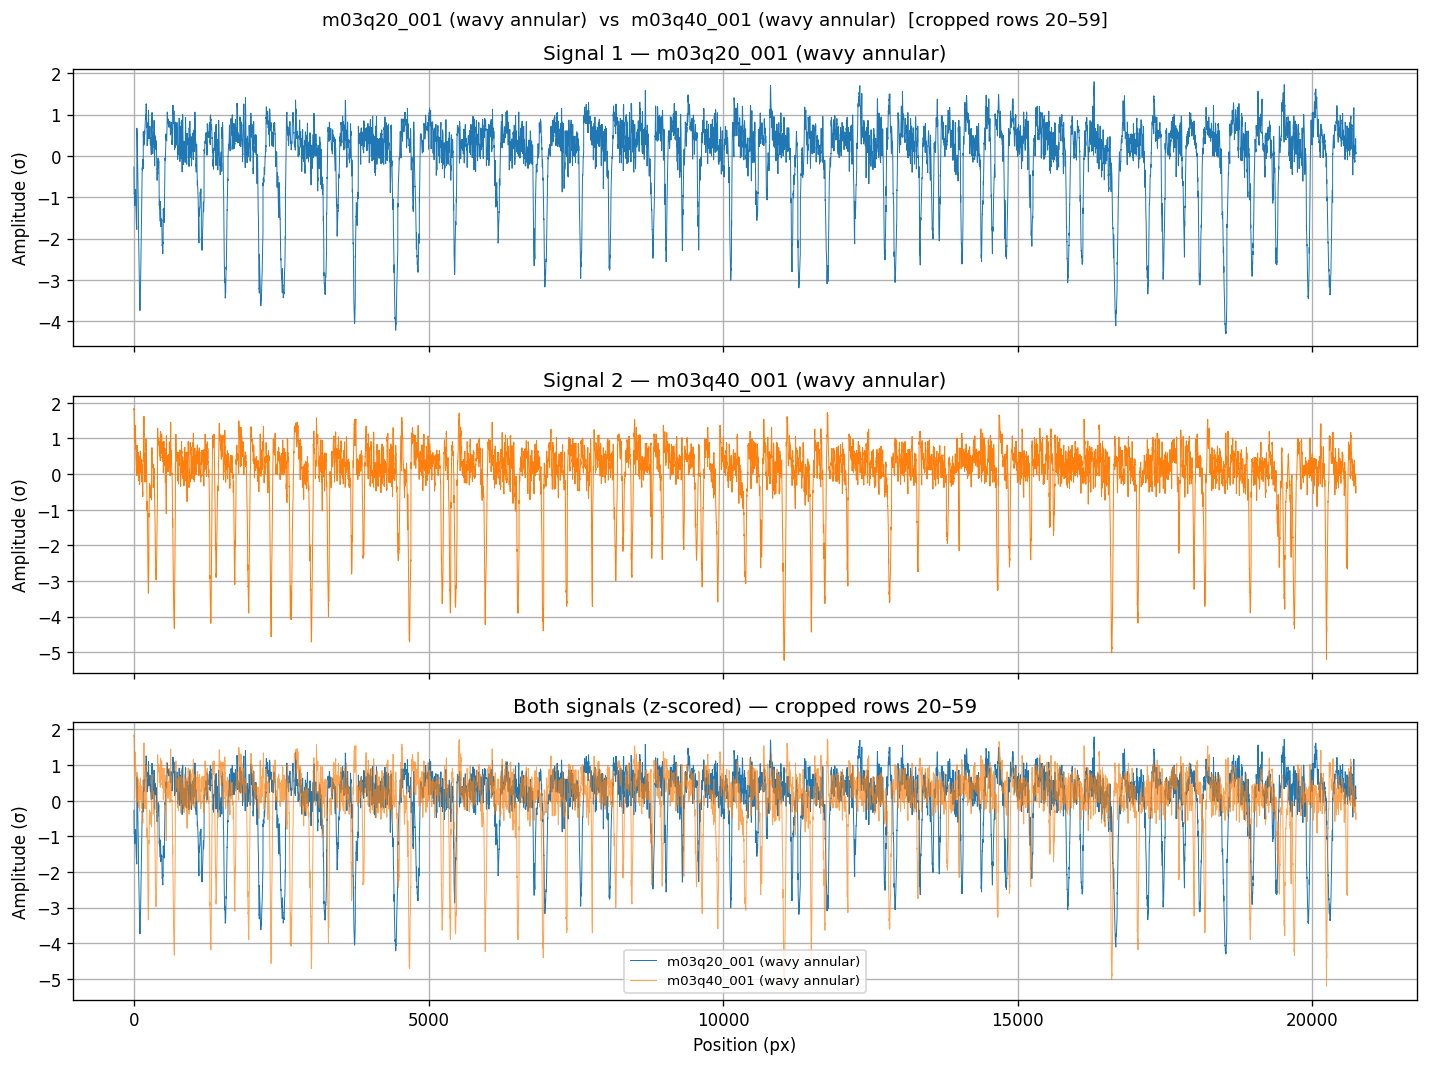
\includegraphics[width=0.92\textwidth]{figuras/v8-annular-signals}
  \caption{Sinais espaciais de brilho de dois ensaios de anular ondulado, na variante
           \textit{cropped}. Mesma disposição de painéis da \autoref{fig:res-sinais}.}
  \label{fig:res-sinais-annular}
  \fonte{Elaborado pelo autor.}
\end{figure}

\begin{figure}[htbp]
  \centering
  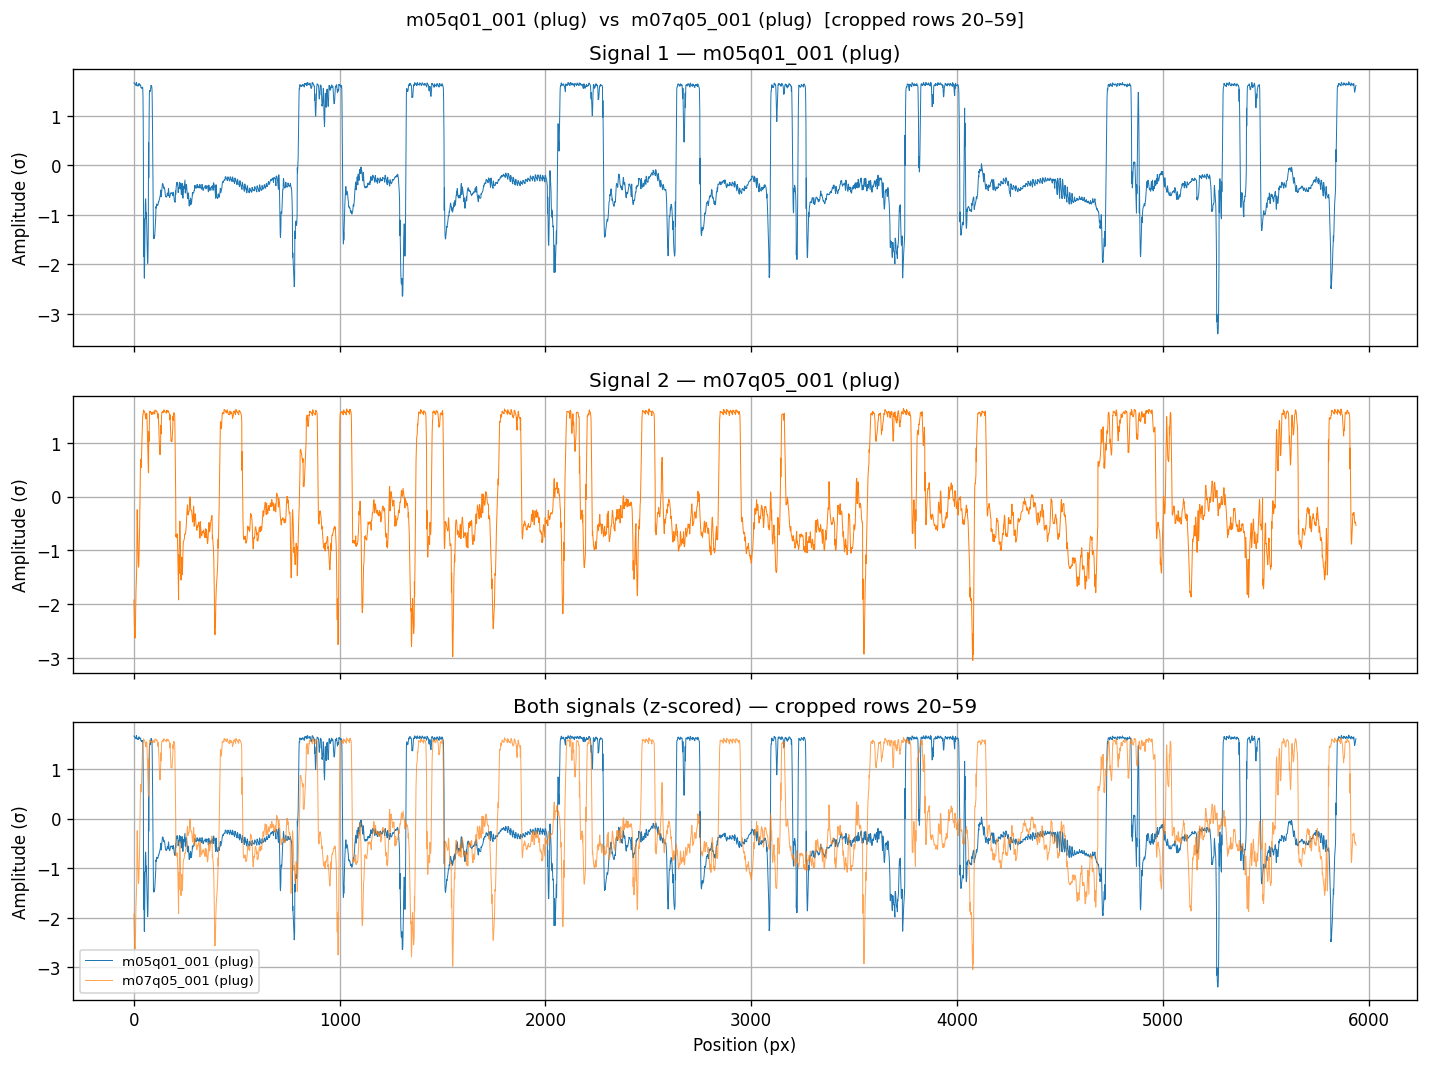
\includegraphics[width=0.92\textwidth]{figuras/v8-plug-signals}
  \caption{Sinais espaciais de brilho de dois ensaios de \textit{plug}, na variante
           \textit{cropped}. Mesma disposição de painéis da \autoref{fig:res-sinais}.}
  \label{fig:res-sinais-plug}
  \fonte{Elaborado pelo autor.}
\end{figure}

\begin{figure}[htbp]
  \centering
  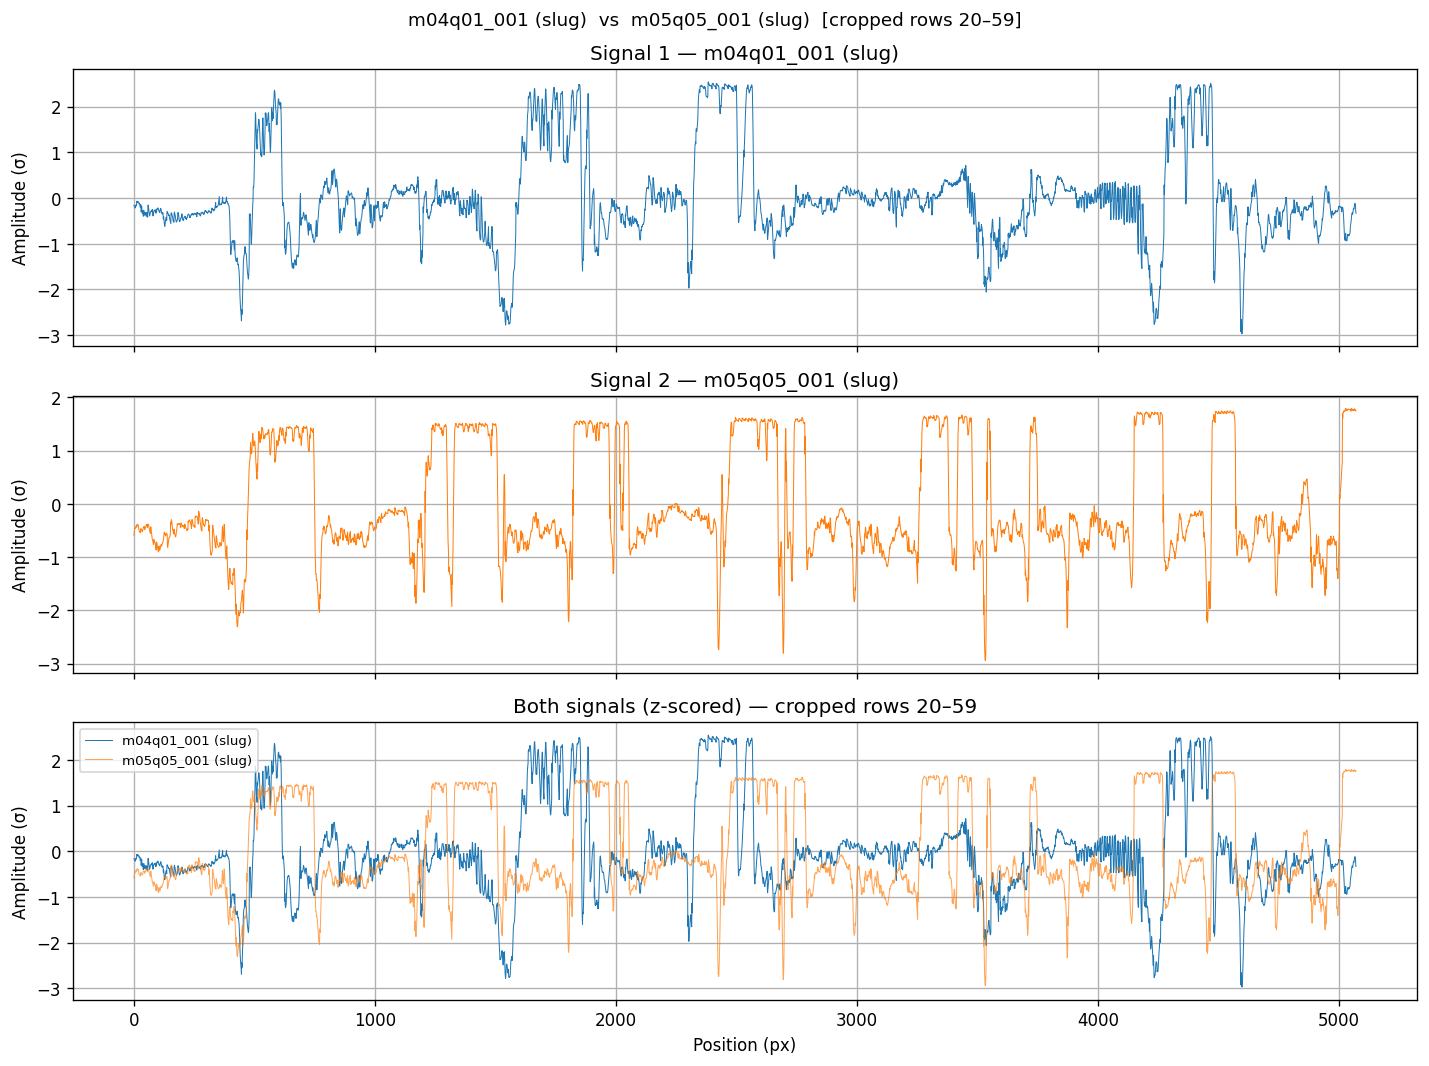
\includegraphics[width=0.92\textwidth]{figuras/v8-slug-signals}
  \caption{Sinais espaciais de brilho de dois ensaios de \textit{slug}, na variante
           \textit{cropped}. Mesma disposição de painéis da \autoref{fig:res-sinais}.}
  \label{fig:res-sinais-slug}
  \fonte{Elaborado pelo autor.}
\end{figure}

% =========================================================
\section{Espectro de potência e perfil de potência média}\label{sec:res-wps}
% =========================================================

Os campos de espectro de potência $\widetilde{P}_x(a)$ e $\widetilde{P}_y(a)$, obtidos da CWT das
funções de autocorrelação de cada ensaio, concentraram sua energia em uma faixa de comprimento de
onda bem delimitada. Em termos simples, a \textit{autocorrelação} mede o quanto o sinal de um
ensaio se parece consigo mesmo quando deslocado ao longo do percurso, revelando os tamanhos de
estrutura (comprimentos de onda) que se repetem no escoamento. A formulação de
\citeonline{schuck2019} parte dessas funções de correlação, e não do sinal bruto. O
\textit{espectro de potência} resultante indica quanta energia o padrão concentra em cada tamanho
de estrutura, e o \textit{perfil de potência média} $|\text{WPS}|$ resume essa informação em uma
única curva, cujo máximo aponta o comprimento de onda dominante do padrão. Nos ensaios de
\textit{churn} e de anular ondulado, essa concentração situou-se
na região de centenas de pixels de comprimento de onda, com o perfil de potência média
$|\text{WPS}|$ exibindo um máximo pronunciado nessa faixa e caindo para os comprimentos de onda mais
curtos e mais longos. Os painéis superiores da \autoref{fig:res-wps} mostram esse comportamento para
dois ensaios de \textit{churn}: os campos WPS apresentam um lóbulo central de magnitude elevada em
torno do atraso nulo, e os perfis de potência média ao lado exibem o pico correspondente na mesma
faixa de comprimento de onda.

\begin{figure}[htbp]
  \centering
  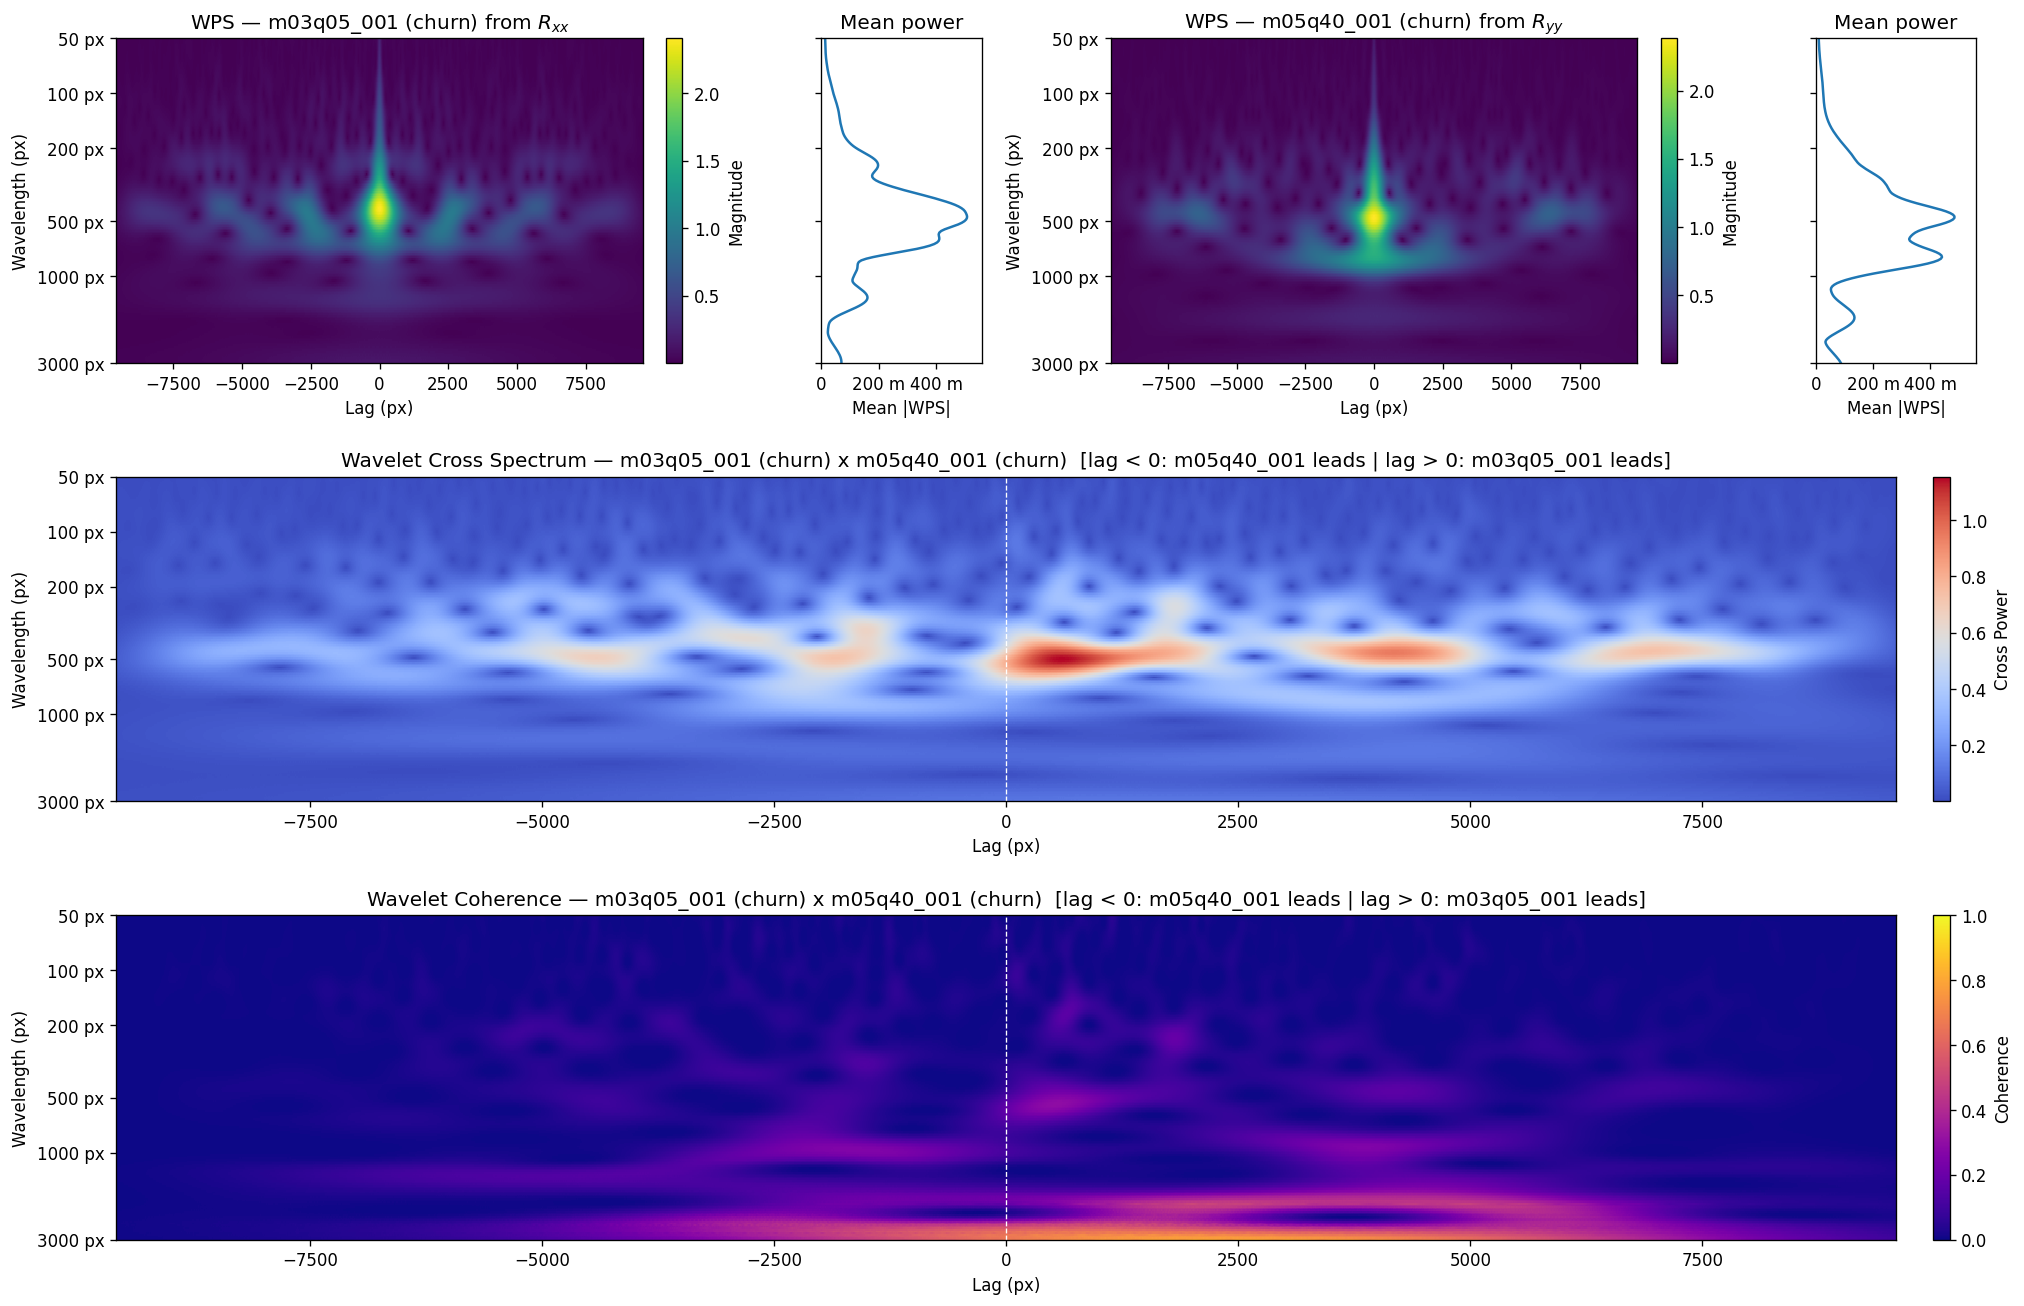
\includegraphics[width=\textwidth]{figuras/v8-churn-churn-wavelet}
  \caption{Campos espectrais de um par de ensaios de \textit{churn} (variante \textit{cropped}).
           Linha superior: espectro de potência $\widetilde{P}_x$ e $\widetilde{P}_y$ de cada
           ensaio, com o respectivo perfil de potência média $|\text{WPS}|$ ao lado. Linha central:
           espectro cruzado $\widetilde{C}_{xy}$. Linha inferior: coerência
           $\widetilde{\gamma}_{xy}$. Eixo vertical em comprimento de onda (pixels), eixo horizontal
           em atraso (pixels).}
  \label{fig:res-wps}
  \fonte{Elaborado pelo autor.}
\end{figure}

Essa faixa dominante mostrou-se a característica mais estável dos campos obtidos. O perfil de
potência média resumiu em uma única curva o comprimento de onda em que a energia espectral de cada
ensaio se concentra, e foi essa curva que apresentou o comportamento mais regular e mais fácil de
comparar entre ensaios, tanto na inspeção intra-padrão quanto na inter-padrão descritas adiante.

Para cada ensaio elegível, extraiu-se o comprimento de onda dominante $\lambda^*$, definido na
\autoref{sec:met-analise} como a posição do máximo do perfil de potência média $|\text{WPS}|$
na variante \textit{cropped}. O \autoref{quad:res-lambda} reúne a faixa de $\lambda^*$ observada em
cada padrão. Os ensaios de anular ondulado concentraram o máximo de potência na faixa mais estreita,
entre cerca de 350 e 570 pixels (mediana em torno de 490 pixels), ao passo que os de \textit{churn}
mantiveram o máximo majoritariamente entre cerca de 430 e 790 pixels (mediana em torno de 630
pixels), com um ensaio isolado deslocado para comprimentos de onda mais longos. Os padrões com
poucos ensaios apresentaram dispersão maior: \textit{plug} espalhou-se entre cerca de 220 e 710
pixels, enquanto \textit{slug} e \textit{slug}--\textit{churn} espalharam-se por uma faixa ampla,
chegando ao limite superior da grade de comprimentos de onda em um dos ensaios, o que reflete o
número reduzido de amostras desses padrões.

\begin{quadro}[htb]
  \centering
  \caption{Comprimento de onda dominante $\lambda^*$ (máximo do perfil de potência média
           $|\text{WPS}|$) por padrão, na variante \textit{cropped}, para os ensaios elegíveis
           de cada padrão. A coluna ``Coerência'' resume a leitura qualitativa da coerência no
           atraso nulo.}
  \label{quad:res-lambda}
  \begin{tabular}{l c c c c}
    \hline
    \textbf{Padrão} & \textbf{Ensaios} & \textbf{Faixa de $\lambda^*$ (px)} & \textbf{Mediana (px)} & \textbf{Coerência} \\
    \hline
    \textit{Churn}                      & 10 & 434--1264 & 629 & baixa/irregular \\
    Anular ondulado                     &  9 & 353--567  & 491 & baixa/irregular \\
    \textit{Plug}                       &  4 & 220--711  & 550 & baixa/irregular \\
    \textit{Slug}                       &  3 & 682--1213 & 711 & baixa/irregular \\
    \textit{Slug}--\textit{churn}       &  2 & 910--3000 & --- & baixa/irregular \\
    \hline
  \end{tabular}
  \fonte{Elaborado pelo autor.}
\end{quadro}

Os demais padrões apresentaram o mesmo arranjo de campos, deslocando apenas a posição da faixa
dominante. A \autoref{fig:res-wps-annular} mostra o par de anular ondulado, cujo perfil de potência
média concentra o máximo na faixa mais estreita e mais curta entre os padrões, em torno de 490
pixels. A \autoref{fig:res-wps-plug} e a \autoref{fig:res-wps-slug} mostram os pares de \textit{plug}
e de \textit{slug}, com o máximo mais disperso e deslocado para comprimentos de onda mais longos,
coerente com o número reduzido de ensaios registrado no \autoref{quad:res-lambda}. Em todos os casos,
a linha inferior de coerência permaneceu escura na maior parte da faixa, sem uma banda que
acompanhasse o máximo de potência, comportamento retomado na \autoref{sec:res-wco}.

\begin{figure}[htbp]
  \centering
  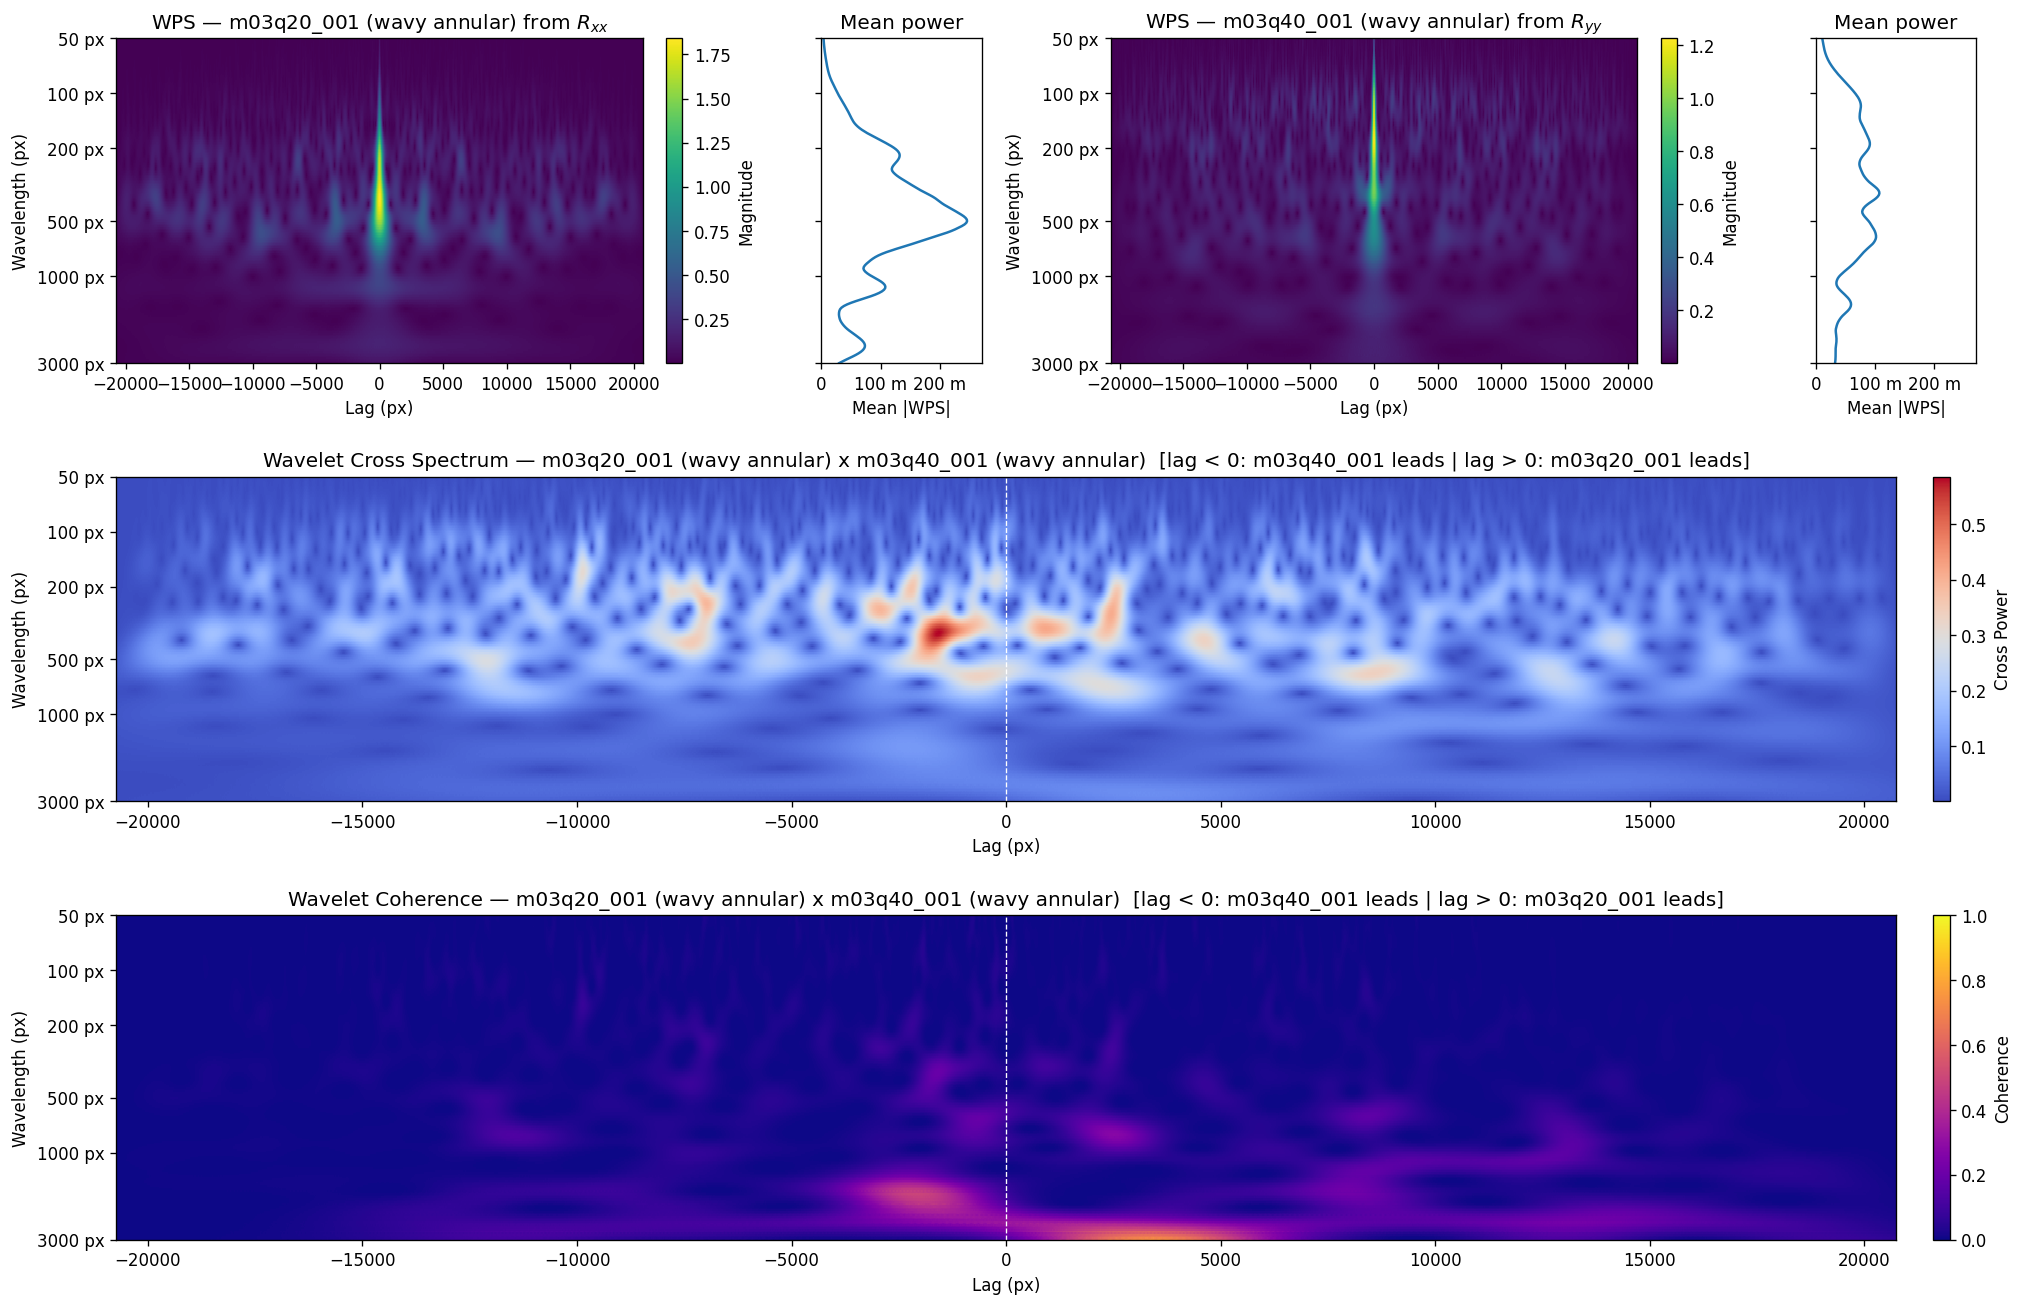
\includegraphics[width=\textwidth]{figuras/v8-annular-wavelet}
  \caption{Campos espectrais de um par de ensaios de anular ondulado (variante \textit{cropped}).
           Mesma disposição de painéis da \autoref{fig:res-wps}. O perfil de potência média
           concentra o máximo na faixa mais estreita e curta entre os padrões.}
  \label{fig:res-wps-annular}
  \fonte{Elaborado pelo autor.}
\end{figure}

\begin{figure}[htbp]
  \centering
  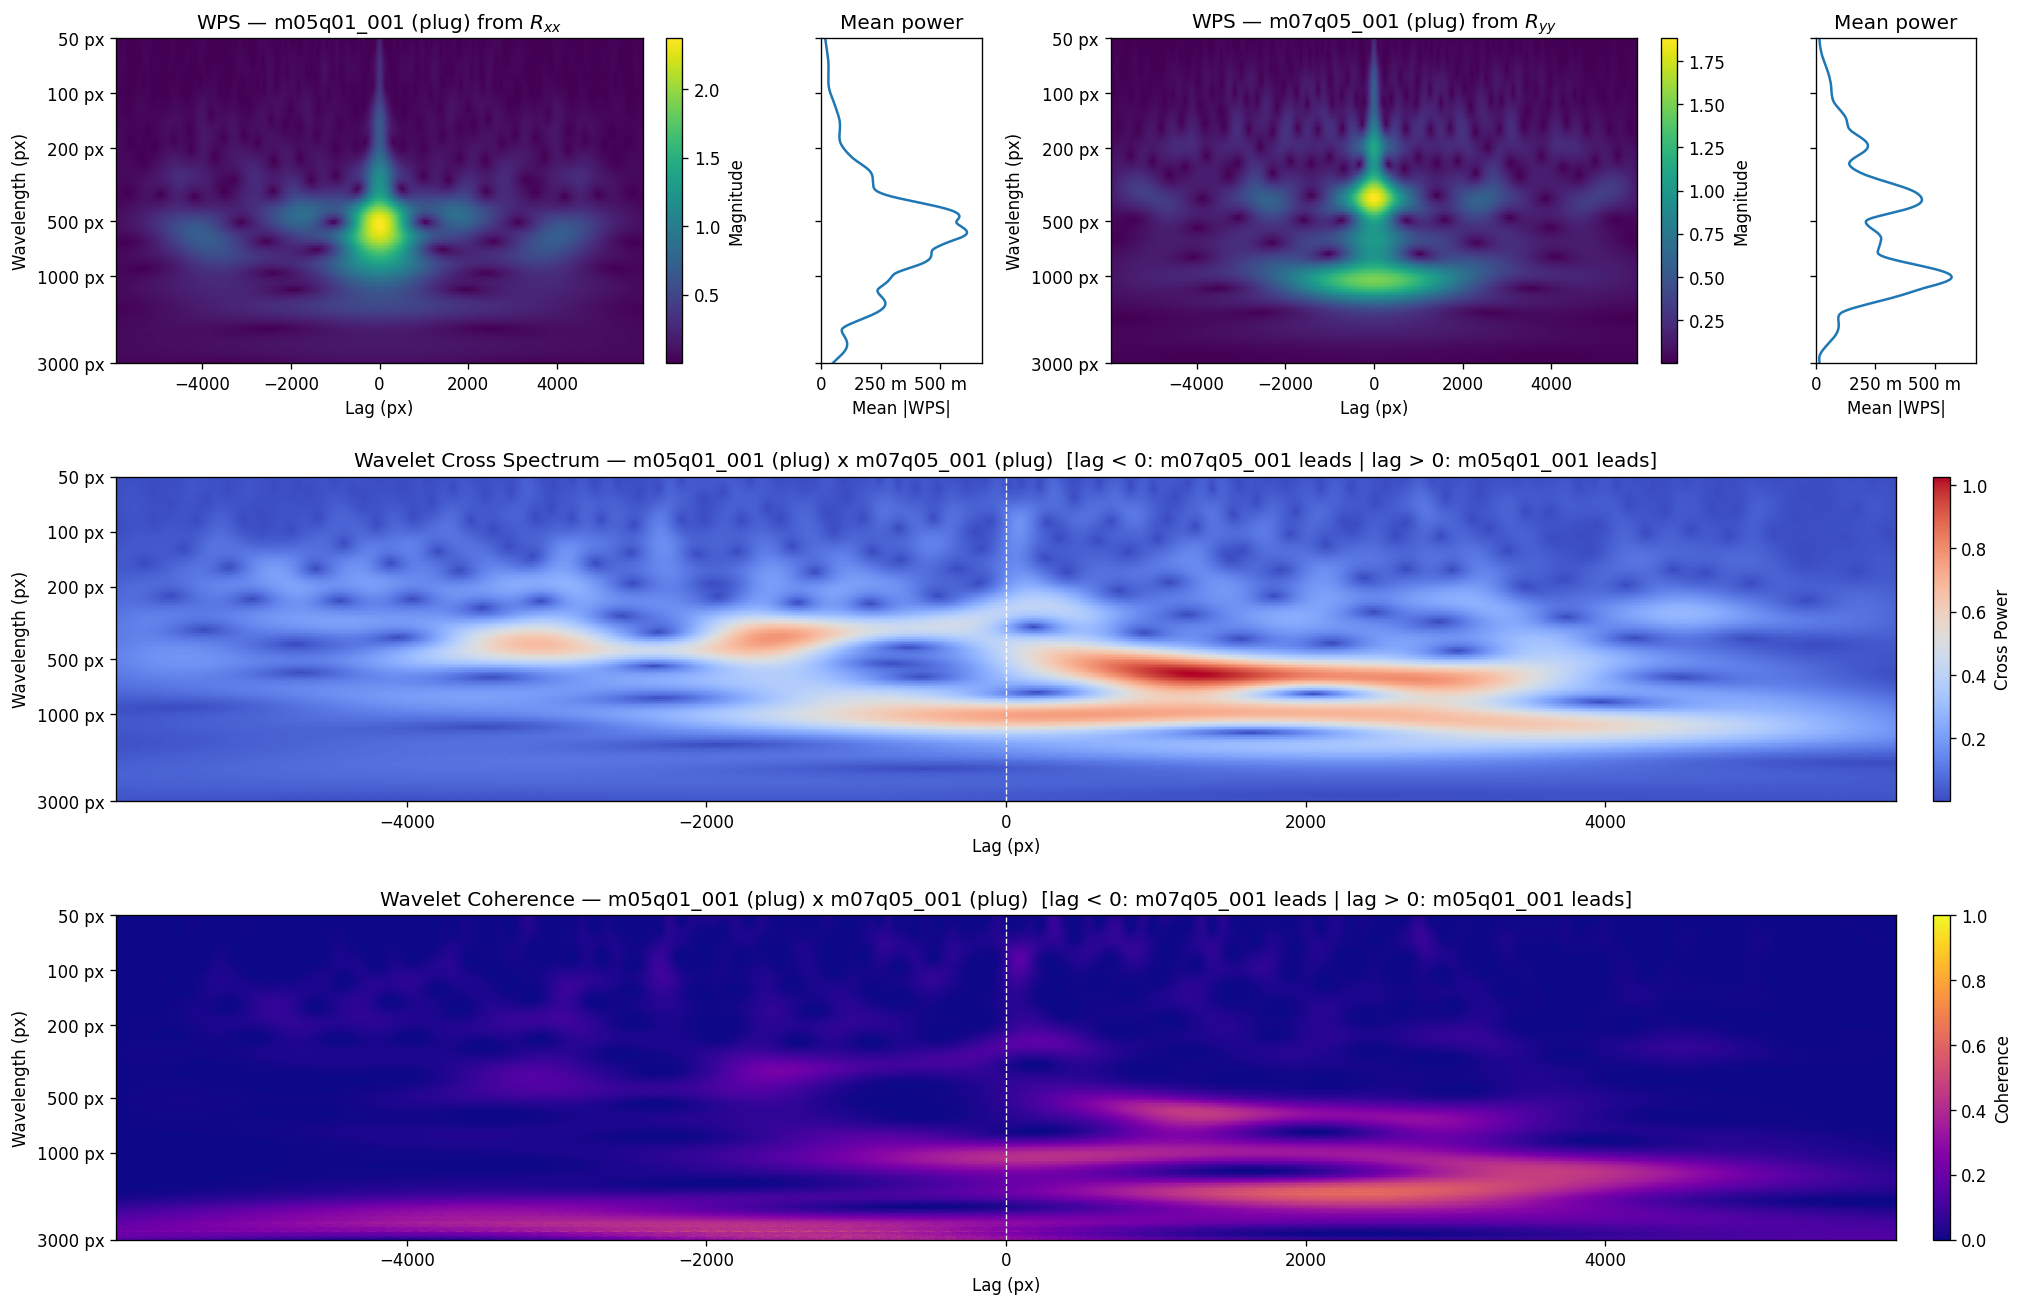
\includegraphics[width=\textwidth]{figuras/v8-plug-wavelet}
  \caption{Campos espectrais de um par de ensaios de \textit{plug} (variante \textit{cropped}).
           Mesma disposição de painéis da \autoref{fig:res-wps}.}
  \label{fig:res-wps-plug}
  \fonte{Elaborado pelo autor.}
\end{figure}

\begin{figure}[htbp]
  \centering
  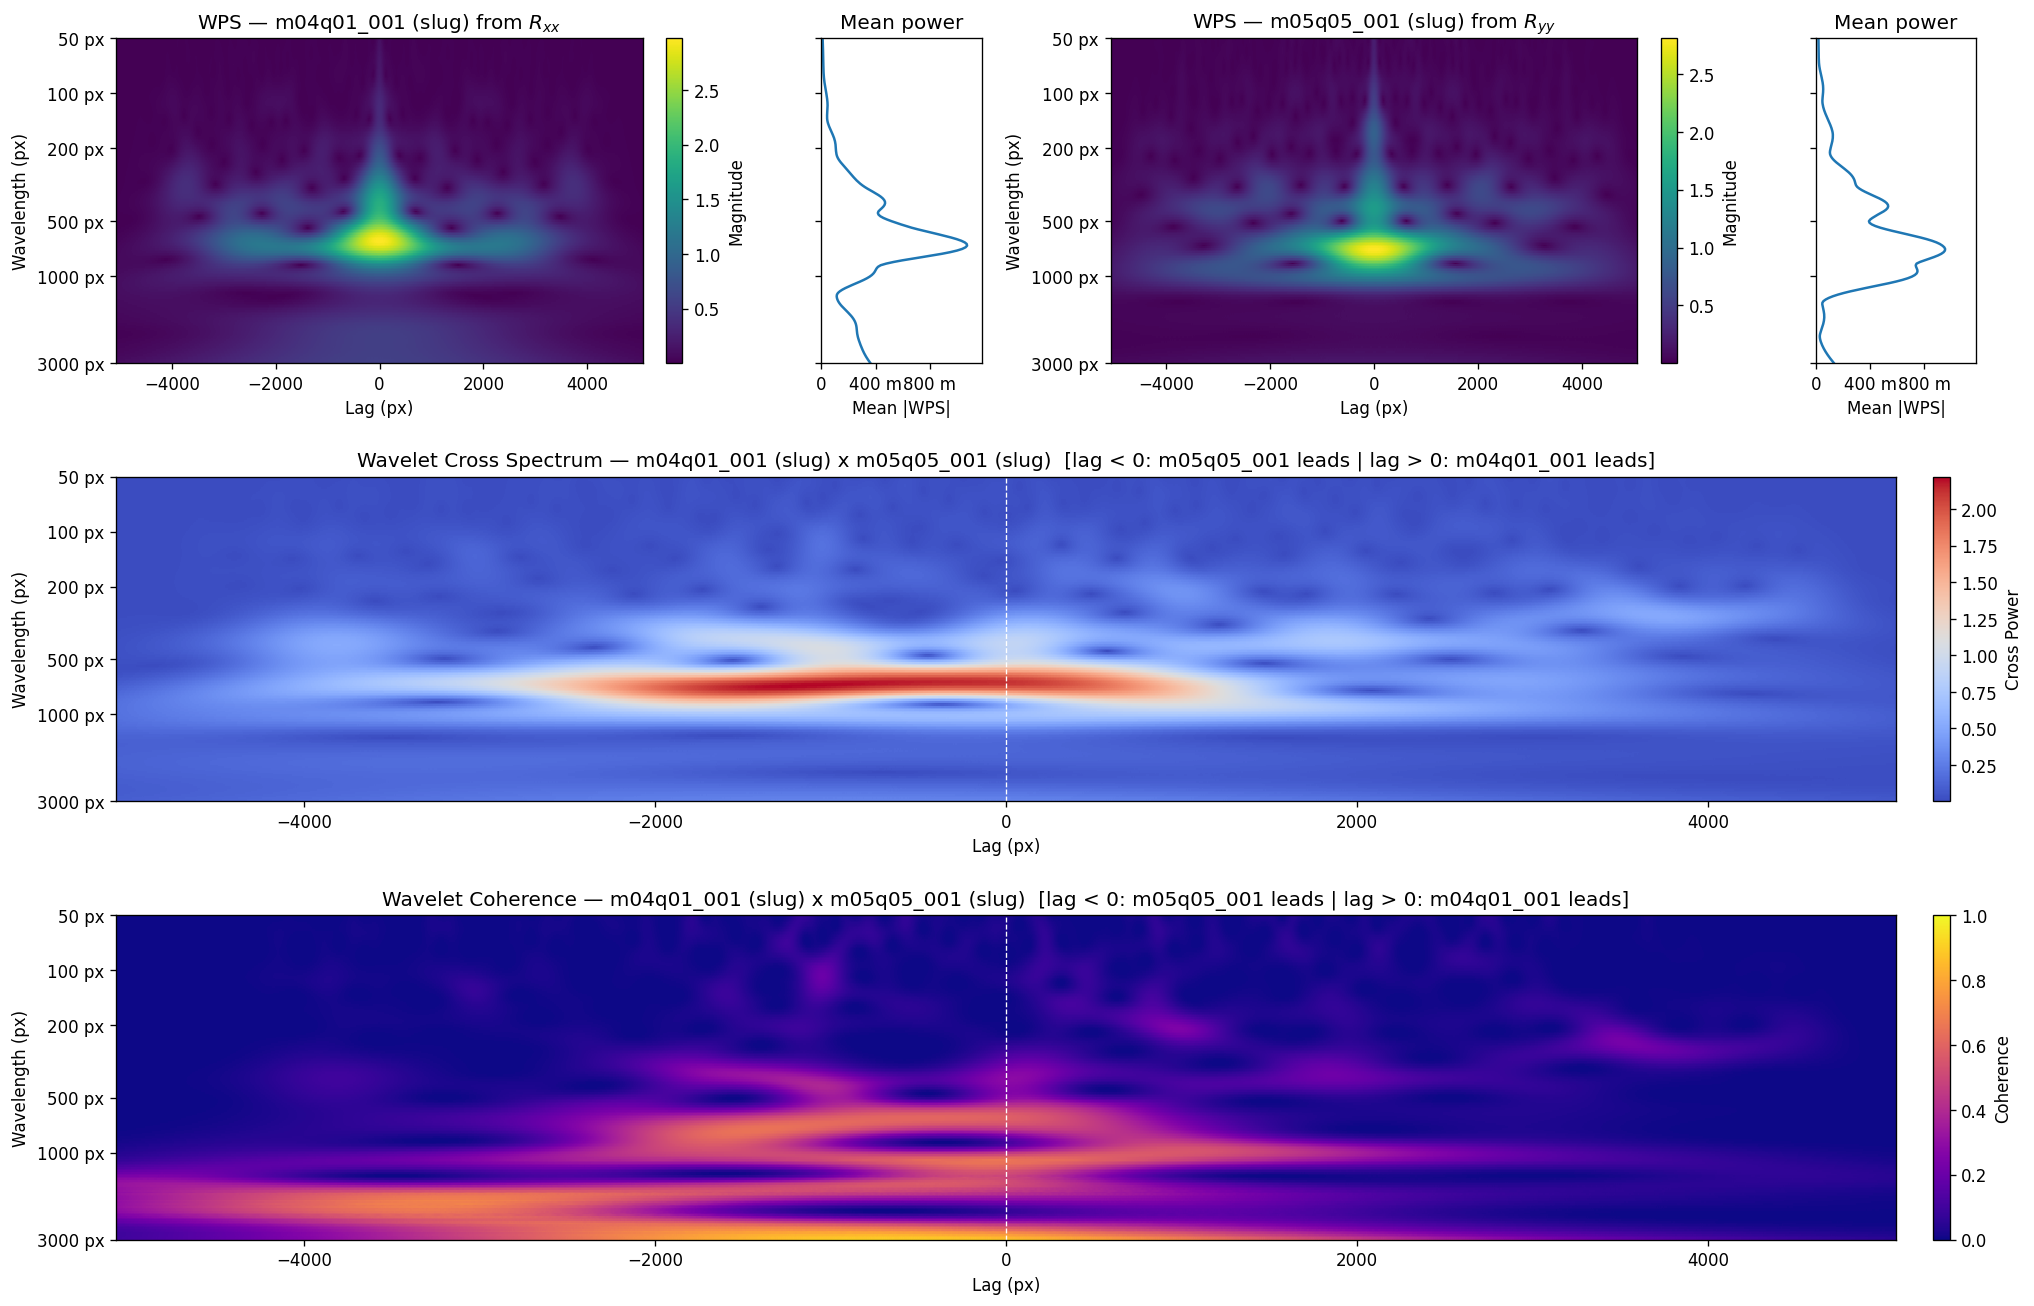
\includegraphics[width=\textwidth]{figuras/v8-slug-wavelet}
  \caption{Campos espectrais de um par de ensaios de \textit{slug} (variante \textit{cropped}).
           Mesma disposição de painéis da \autoref{fig:res-wps}.}
  \label{fig:res-wps-slug}
  \fonte{Elaborado pelo autor.}
\end{figure}

% =========================================================
\section{Campo de coerência \textit{Wavelet} alternativa}\label{sec:res-wco}
% =========================================================

O campo de coerência $\widetilde{\gamma}_{xy}(a)$, descritor principal deste trabalho, foi obtido
para todos os pares das duas campanhas. Antes de descrever o que se observou, convém explicar o
que cada campo representa. O \textit{espectro cruzado} (WCS) mede a energia que os dois ensaios
têm em comum em cada tamanho de estrutura. A \textit{coerência} (WCO), derivada dele, varia de
zero a um e indica o quanto os dois ensaios ``andam juntos'' em cada comprimento de onda, no
atraso nulo. A expectativa era de que dois ensaios de um mesmo padrão, por compartilharem o mesmo
tipo de estrutura, apresentassem coerência elevada na faixa dominante. Na inspeção dos campos, a
coerência avaliada no atraso nulo
apresentou-se em geral baixa e irregular ao longo dos comprimentos de onda, mesmo entre ensaios de
um mesmo padrão. Os valores de coerência mais altos concentraram-se nos comprimentos de onda
mais longos, nos quais a largura finita do campo abrange poucos períodos espaciais e a coerência
fica mal determinada. Por isso, a coerência elevada observada nessa região de ondas longas não
constitui evidência de acoplamento entre os ensaios. A linha inferior da \autoref{fig:res-wps} ilustra esse comportamento para o par de
ensaios de \textit{churn}: o campo de coerência permanece escuro na maior parte da faixa de
comprimentos de onda em torno do atraso nulo, sem uma banda de coerência elevada que acompanhe a
faixa dominante identificada nos perfis de potência média.

Esse resultado indica que a coerência \textit{Wavelet} alternativa, tomada no atraso nulo entre
pares de ensaios, não descreveu os padrões de escoamento com a precisão esperada para o arranjo e os
sinais utilizados. A caracterização mais consistente veio do perfil de potência média
$|\text{WPS}|$, cujo comportamento é retomado nas comparações a seguir.

% =========================================================
\section{Repetibilidade intra-padrão}\label{sec:res-intra}
% =========================================================

Na campanha intra-padrão, os campos de vários pares de ensaios de um mesmo padrão foram comparados
entre si. Os perfis de potência média $|\text{WPS}|$ dos ensaios de anular ondulado apresentaram o
comprimento de onda dominante na faixa mais concentrada entre os padrões, conforme o
\autoref{quad:res-lambda}, indicando que a posição do máximo de potência é a característica mais
reprodutível desse padrão. Os ensaios de \textit{churn} mantiveram o máximo na mesma ordem de
grandeza de um ensaio para outro, porém com dispersão maior, incluindo um ensaio com o máximo
deslocado para comprimentos de onda mais longos. Em ambos os padrões, a posição do máximo de potência
repetiu-se de forma mais evidente do que qualquer característica do campo de coerência. Os padrões
com menos ensaios (\textit{plug}, \textit{slug} e \textit{slug}--\textit{churn}) foram examinados de
forma ilustrativa, por disporem de poucos pares, e exibiram dispersão ainda maior do comprimento de
onda dominante, conforme os campos das \autoref{fig:res-wps-plug} e \autoref{fig:res-wps-slug}.

O campo de coerência $\widetilde{\gamma}_{xy}(a)$, por sua vez, não reproduziu essa regularidade:
entre pares de ensaios de um mesmo padrão a coerência no atraso nulo permaneceu baixa e sem uma banda
estável, de modo que a repetibilidade intra-padrão ficou muito mais evidente no perfil de potência
média do que no campo de coerência.

% =========================================================
\section{Separação inter-padrão}\label{sec:res-inter}
% =========================================================

Na campanha inter-padrão, os campos de pares de ensaios de padrões distintos foram comparados para
verificar se as assinaturas espectrais se distinguem de um padrão para outro. A
\autoref{fig:res-inter} mostra um par formado por um ensaio de \textit{churn} e um de anular
ondulado. Os perfis de potência média dos dois ensaios apresentaram faixas dominantes parcialmente
sobrepostas, na mesma ordem de comprimento de onda, de modo que a separação entre os dois padrões
por esse descritor mostrou-se sutil. Essa sobreposição é coerente com as faixas de comprimento de
onda dominante do \autoref{quad:res-lambda}: a faixa do anular ondulado está contida na faixa mais
ampla do \textit{churn}, de modo que o comprimento de onda dominante, isoladamente, não separa os
dois padrões, apenas desloca a mediana de um em relação ao outro. Os ensaios intermitentes de
\textit{plug} e de \textit{slug}, examinados de forma ilustrativa por disporem de poucos ensaios,
situam o comprimento de onda dominante em valores em geral mais longos e mais dispersos do que os
de anular ondulado, coerente com estruturas maiores e mais espaçadas; essa leitura, porém, apoia-se
em um número reduzido de ensaios e não sustenta uma separação inter-padrão firme. O campo de
coerência no atraso nulo, novamente baixo e irregular, não forneceu uma distinção nítida entre os
padrões.

\begin{figure}[htbp]
  \centering
  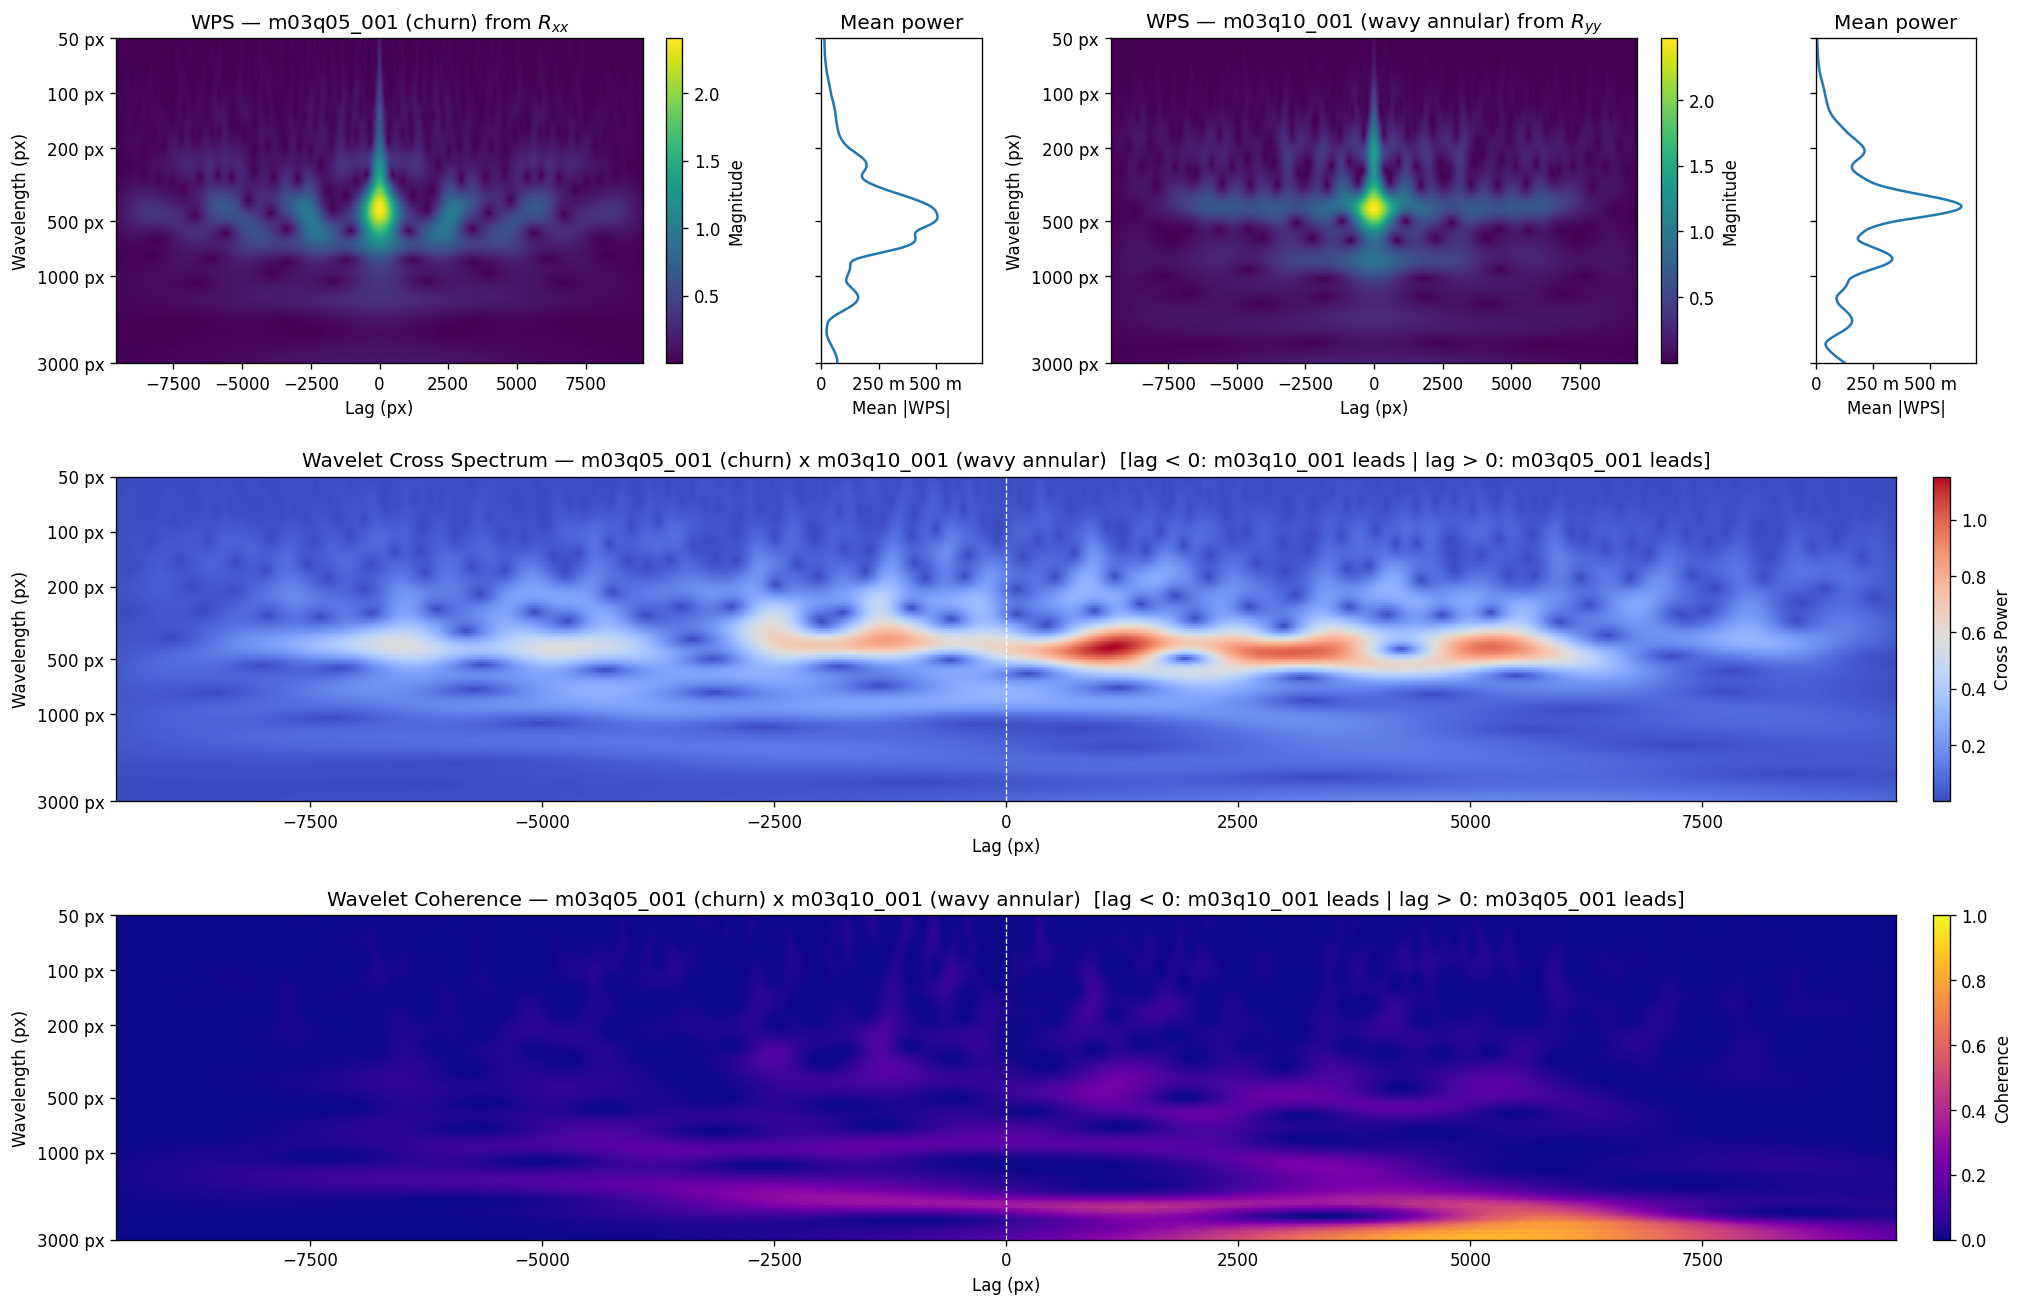
\includegraphics[width=\textwidth]{figuras/v8_1-churn-annular-wavelet}
  \caption{Campos espectrais de um par inter-padrão, um ensaio de \textit{churn} e um de anular
           ondulado (variante \textit{cropped}). Mesma disposição de painéis da
           \autoref{fig:res-wps}. Os perfis de potência média apresentam faixas dominantes
           parcialmente sobrepostas entre os dois padrões.}
  \label{fig:res-inter}
  \fonte{Elaborado pelo autor.}
\end{figure}

As combinações entre padrões foram inspecionadas de forma sistemática, abrangendo os duzentos e
oitenta e sete pares formados pelo produto dos ensaios de cada par de padrões (\textit{churn},
anular ondulado, \textit{plug}, \textit{slug} e \textit{slug}--\textit{churn}). O comportamento
ilustrado na \autoref{fig:res-inter} repetiu-se nas demais combinações: a coerência no atraso nulo
manteve-se baixa e irregular, sem distinção nítida entre padrões, e as faixas dominantes de
$\lambda^*$ apresentaram apenas sobreposição parcial. Cada par foi registrado como figura no
conjunto de resultados, o que assegura a rastreabilidade da inspeção visual, embora não se tenham
extraído descritores numéricos por par.

A quantificação da separação entre padrões em nível de ensaio é apresentada na
\autoref{sec:res-limite-estat}, em que a matriz de distância espectral e o teste ANOSIM fornecem a
evidência estatística correspondente. Ela abrange os quatro padrões com mais de dois ensaios
(\textit{churn}, anular ondulado, \textit{plug} e \textit{slug}); o \textit{slug}--\textit{churn},
com apenas dois ensaios, permaneceu de caráter ilustrativo.

% =========================================================
\section{Quantificação estatística da repetibilidade}\label{sec:res-limite-estat}
% =========================================================

A leitura qualitativa dos campos foi complementada por uma quantificação estatística da
repetibilidade do descritor espectral, destinada a medir objetivamente o quanto ensaios de um mesmo
padrão de escoamento se parecem entre si em comparação com ensaios de padrões diferentes. Essa
quantificação confirma e dimensiona o que a inspeção visual já indicava: a semelhança intra-padrão
existe, mas é sutil --- não uma distinção evidente, como a que separa duas classes de objetos
claramente distintas, e sim uma semelhança modesta, do tipo que se percebe entre dois exemplares
aparentados, com um ``ar de família'' acompanhado de considerável variação dentro de cada grupo. A
análise abrangeu os quatro padrões com mais de dois ensaios, \textit{churn} (dez ensaios), anular
ondulado (nove), \textit{plug} (quatro) e \textit{slug} (três), totalizando vinte e seis ensaios; o
\textit{slug}--\textit{churn}, com apenas dois ensaios, ficou de fora por não sustentar uma leitura
de grupo. As subseções a seguir apresentam, de forma didática, o propósito de cada etapa, o
resultado esperado e o que de fato se obteve.

% ---------------------------------------------------------
\subsection{Métrica de distância espectral entre ensaios}\label{sec:res-estat-distancia}
% ---------------------------------------------------------

O descritor submetido à análise não foi o campo de coerência, mas o perfil de potência média
$|\text{WPS}|$ por ensaio, que foi a característica mais reprodutível identificada na inspeção dos
campos. Para cada ensaio tomou-se o perfil de potência média na coluna de atraso nulo, branqueado
por escala pela remoção do decaimento espectral comum de fundo, de modo que o descritor retenha a
\emph{forma} do espectro, isto é, em quais tamanhos de estrutura a energia se concentra, e não a sua
amplitude bruta. Para que todos os ensaios tenham o mesmo comprimento, as séries foram truncadas ao
tamanho do menor ensaio de \textit{churn}. Por essa razão, o descritor usado aqui difere do perfil
de potência média de sinal completo que originou o comprimento de onda dominante $\lambda^*$ do
\autoref{quad:res-lambda}, cujos valores não devem ser lidos como entrada direta do teste.

A semelhança entre dois ensaios foi medida pela \emph{correlação de Pearson} entre seus perfis: um
número que resume o quanto duas curvas sobem e descem juntas, próximo de um quando têm a mesma forma
e próximo de zero quando não guardam relação. A partir dela define-se a \emph{distância} entre dois
ensaios $i$ e $j$ como um menos essa correlação,

\begin{equation}\label{eq:dist-pearson}
  d_{ij} = 1 - \rho(\mathbf{z}_i, \mathbf{z}_j),
\end{equation}

\noindent em que $\mathbf{z}_i$ e $\mathbf{z}_j$ são os perfis de potência branqueados dos dois
ensaios e $\rho$ é a correlação de Pearson entre eles. Em termos do cálculo, $\rho$ compara os dois
perfis frequência a frequência: para cada frequência verifica se os dois ensaios estão
simultaneamente acima ou abaixo da sua própria energia média e, somando essas concordâncias ao longo
de todo o espectro, resume em um único número se as duas curvas sobem e descem em sintonia. Vale
próximo de um quando os perfis têm picos e vales nas mesmas frequências (mesma forma espectral), em
torno de zero quando não há relação entre eles e torna-se negativo quando têm formas opostas --- um
com pico onde o outro tem vale ---, caso em que a distância da \autoref{eq:dist-pearson} ultrapassa a
unidade. Por depender apenas da forma relativa das curvas, e não de sua amplitude bruta, $\rho$ é
insensível à escala de energia de cada ensaio. Assim, ensaios de forma idêntica têm distância
nula e ensaios sem relação têm distância próxima de um. Calculando essa distância para todos os pares
obtém-se uma matriz de distâncias entre os vinte e seis ensaios, representada no
\autoref{fig:res-dmatrix}. Nela, os blocos na diagonal reúnem os ensaios de um mesmo padrão. A
predominância de tons mais claros (menor distância) nesses blocos, em relação aos blocos fora da
diagonal, é a manifestação visual da semelhança intra-padrão que a análise quantifica. Chama a
atenção um ensaio de \textit{plug} (o ensaio 21) cujas linha e coluna são escuras em quase toda a
extensão: sua assinatura espectral é atípica, anticorrelacionada com a da maioria dos demais
ensaios. Trata-se de variação real desse ensaio, mantida na análise e não removida, e explica em
parte por que o grupo \textit{plug} é internamente heterogêneo.

\begin{figure}[htbp]
  \centering
  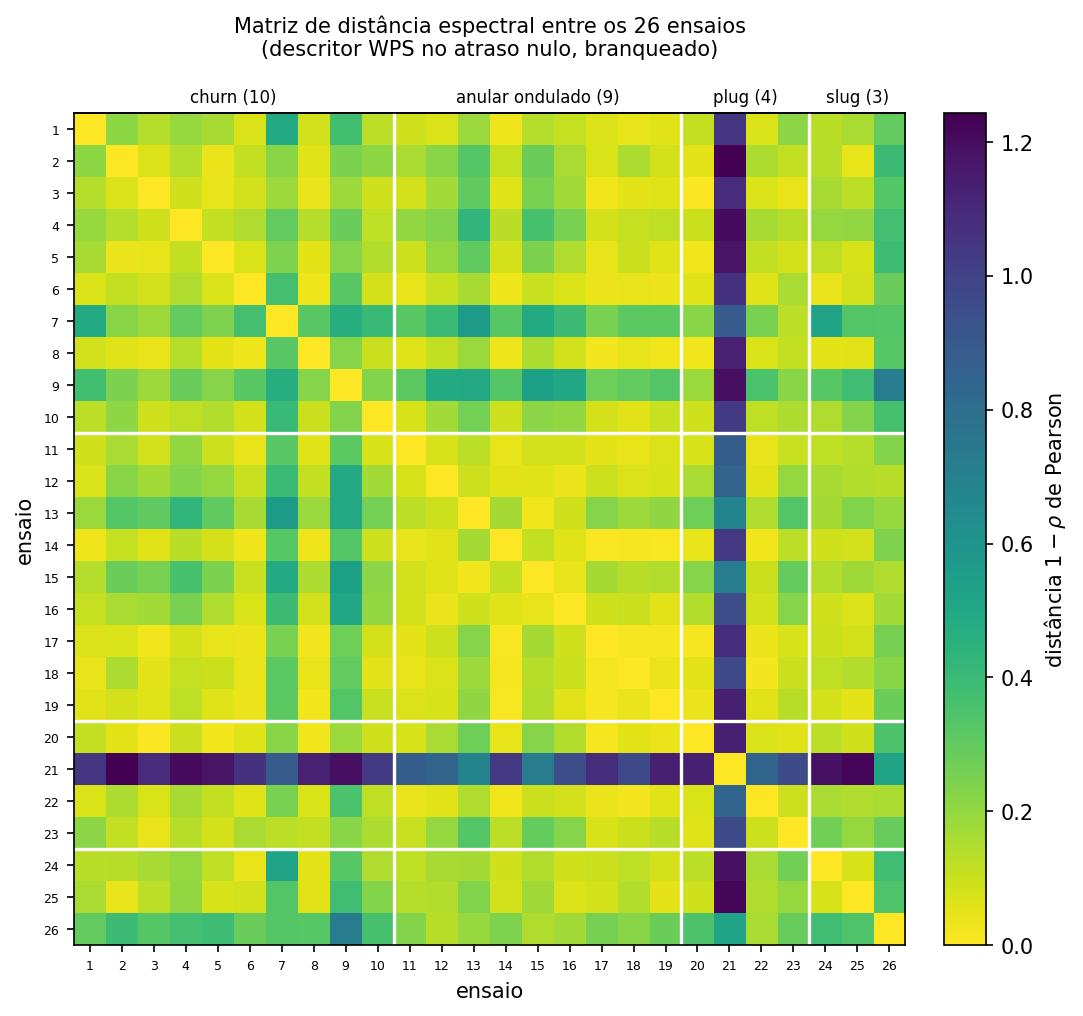
\includegraphics[width=0.78\textwidth]{figuras/v8-estat-dmatrix}
  \caption{Matriz de distância espectral ($1$ menos a correlação de Pearson entre os perfis de
           potência branqueados) entre os vinte e seis ensaios, ordenados por padrão
           (\textit{churn}, ensaios 1 a 10; anular ondulado, 11 a 19; \textit{plug}, 20 a 23;
           \textit{slug}, 24 a 26). Cores mais claras indicam ensaios mais parecidos; as linhas
           brancas separam os quatro padrões, e os blocos na diagonal correspondem a pares de um
           mesmo padrão. A cruz escura no ensaio 21 (um \textit{plug}) assinala um ensaio de
           assinatura atípica, anticorrelacionado com quase todos os demais.}
  \label{fig:res-dmatrix}
  \fonte{Elaborado pelo autor.}
\end{figure}

% ---------------------------------------------------------
\subsection{Teste de similaridade entre grupos (ANOSIM)}\label{sec:res-estat-anosim}
% ---------------------------------------------------------

Sobre a matriz de distâncias aplicou-se o coeficiente $R$ de ANOSIM, um teste simples de
comparação entre grupos. Ele ordena todas as $M = \binom{n}{2}$ distâncias da menor para a maior,
atribuindo a cada uma um posto, e compara o posto médio das distâncias ``mesmo padrão'' com o das
distâncias ``padrões diferentes'' por meio do coeficiente

\begin{equation}\label{eq:anosim-r}
  R = \frac{\bar{r}_{\text{entre}} - \bar{r}_{\text{dentro}}}{M/2},
\end{equation}

\noindent em que $\bar{r}_{\text{entre}}$ e $\bar{r}_{\text{dentro}}$ são os postos médios das
distâncias entre padrões distintos e dentro de um mesmo padrão, respectivamente, e $M = \binom{n}{2}$
é o número total de pares de distâncias entre os $n$ ensaios.

O cálculo dos dois postos médios parte de uma única ordenação e segue três passos:

\begin{enumerate}
  \item \textbf{Ranquear.} Todas as $M$ distâncias da matriz são ordenadas em conjunto, sem
        distinguir sua natureza: a menor recebe o posto $1$, a seguinte o posto $2$, e assim por
        diante até a maior, que recebe o posto $M$.
  \item \textbf{Rotular.} Cada par é então classificado conforme os ensaios que o compõem ---
        ``mesmo padrão'', quando ambos pertencem ao mesmo regime, ou ``padrões diferentes'', caso
        contrário.
  \item \textbf{Comparar.} Calcula-se a média dos \emph{postos} (não das distâncias) em cada grupo,
        obtendo $\bar{r}_{\text{dentro}}$ e $\bar{r}_{\text{entre}}$, e toma-se a diferença entre as
        duas.
\end{enumerate}

\noindent Por operar sobre postos, e não sobre os valores absolutos das distâncias, o coeficiente é
insensível à escala da métrica. A diferença $\bar{r}_{\text{entre}} - \bar{r}_{\text{dentro}}$ mede,
então, o quanto os pares de mesmo padrão se concentram entre as menores distâncias da matriz: se os
ensaios de um mesmo regime forem sistematicamente os mais próximos, esses pares ocupam os postos
baixos, $\bar{r}_{\text{dentro}}$ fica pequeno e a diferença torna-se positiva; se o rótulo não tiver
relação com a distância, os dois postos médios se igualam e a diferença se anula. O denominador
$M/2$ é apenas o fator que normaliza essa diferença para o intervalo $[-1, 1]$, correspondendo ao
valor máximo que o numerador pode assumir sob separação perfeita.

O coeficiente $R$ vale próximo de zero quando os dois grupos são indistinguíveis e próximo
de um quando os ensaios de um mesmo padrão são sistematicamente mais próximos entre si do que os de
padrões diferentes. Esperava-se um valor alto, caso os padrões se separassem bem pelo descritor
espectral. O valor observado, tomando os quatro padrões em conjunto, foi $R = 0{,}20$, indicando que
ensaios de um mesmo padrão são, em média, apenas \emph{modestamente} mais próximos entre si do que
ensaios de padrões distintos. Esse valor é coerente com o \autoref{fig:res-estat-ecdf}, que mostra as
distribuições acumuladas empíricas (ECDF) das distâncias intra-padrão e inter-padrão. A ECDF é a
curva que, para cada valor de distância no eixo horizontal, informa a fração de pares de ensaios
com distância menor ou igual a esse valor, de modo que a curva deslocada para a esquerda indica
distâncias sistematicamente menores. A curva intra-padrão situa-se de forma consistente à esquerda
da inter-padrão, com as distâncias de mesmo padrão sistematicamente menores, embora o deslocamento
entre as duas curvas seja pequeno.

\begin{figure}[htbp]
  \centering
  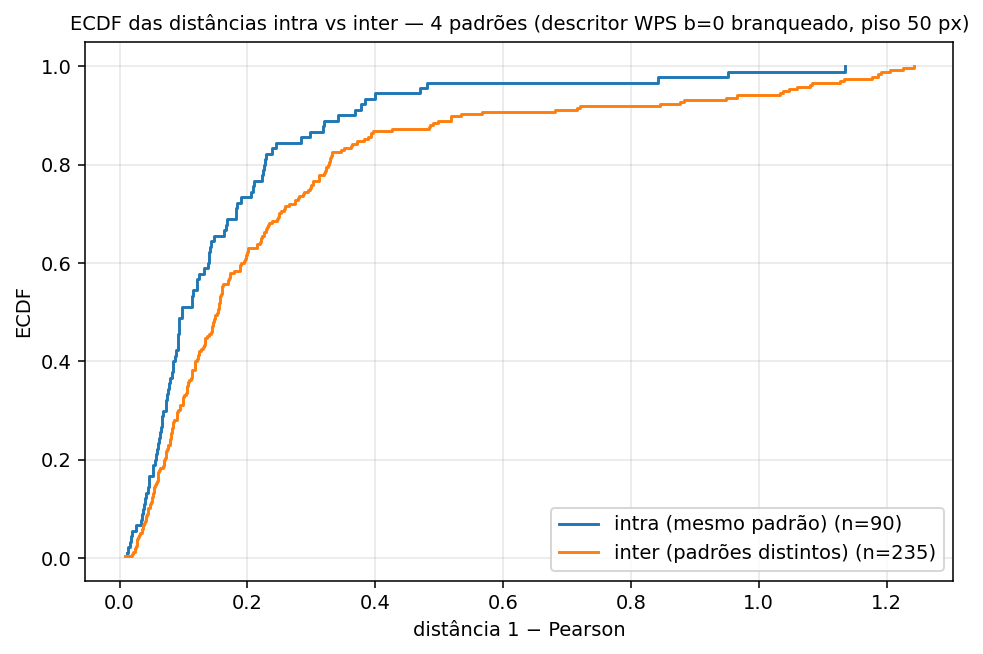
\includegraphics[width=0.82\textwidth]{figuras/v8-estat-ecdf}
  \caption{Distribuição acumulada (ECDF) das distâncias espectrais entre ensaios: dentro de um
           mesmo padrão (\textit{intra}, noventa pares) e entre padrões distintos (\textit{inter},
           duzentos e trinta e cinco pares). A curva intra-padrão, deslocada para a esquerda,
           traduz a separação sutil quantificada por $R = 0{,}20$.}
  \label{fig:res-estat-ecdf}
  \fonte{Elaborado pelo autor.}
\end{figure}

Com quatro padrões, um único coeficiente global esconde quais padrões de fato se separam. Por isso
calculou-se também o $R$ de ANOSIM para cada um dos seis pares de padrões, restringindo a matriz aos
dois grupos de cada vez. O \autoref{quad:res-anosim-pares} reúne esses valores. A leitura par-a-par
revela uma estrutura clara: o anular ondulado é o padrão mais distinto, separando-se bem de todos os
regimes mais lentos, com o maior $R$ de todos frente ao \textit{slug} ($0{,}52$) e separação clara
frente ao \textit{plug} ($0{,}32$). O \textit{slug} é o padrão intermitente que mais contrasta, tanto
com o anular quanto com o \textit{churn} ($0{,}22$). Em contrapartida, \textit{churn} e \textit{plug}
são praticamente indistinguíveis por este descritor ($R = 0{,}03$), e a separação entre \textit{churn}
e anular ondulado permanece fraca ($0{,}18$), reproduzindo o valor já observado quando apenas esses
dois padrões eram comparados. O par \textit{plug}--\textit{slug} ($0{,}11$) apoia-se em poucos pares
de ensaios e deve ser lido com cautela.

\begin{quadro}[htb]
  \centering
  \caption{Coeficiente $R$ de ANOSIM par-a-par entre os quatro padrões, calculado restringindo a
           matriz de distância aos dois grupos de cada par.}
  \label{quad:res-anosim-pares}
  \begin{tabular}{@{}p{0.40\textwidth} c c p{0.28\textwidth}@{}}
    \hline
    \textbf{Par de padrões} & \textbf{$R$} & \textbf{Pares} & \textbf{Leitura} \\
    \hline
    anular ondulado $\times$ \textit{slug}  & $0{,}52$ & 66  & separação mais forte \\
    anular ondulado $\times$ \textit{plug}  & $0{,}32$ & 78  & separação clara \\
    \textit{churn} $\times$ \textit{slug}   & $0{,}22$ & 78  & separação moderada \\
    \textit{churn} $\times$ anular ondulado & $0{,}18$ & 171 & fraca \\
    \textit{plug} $\times$ \textit{slug}    & $0{,}11$ & 21  & fraca, $n$ pequeno \\
    \textit{churn} $\times$ \textit{plug}   & $0{,}03$ & 91  & praticamente indistinguíveis \\
    \hline
  \end{tabular}
  \fonte{Elaborado pelo autor.}
\end{quadro}

% ---------------------------------------------------------
\subsection{Significância por teste de permutação}\label{sec:res-estat-permuta}
% ---------------------------------------------------------

Para avaliar se um $R$ dessa magnitude poderia surgir por acaso, construiu-se uma ``régua do
acaso'' por reamostragem: embaralham-se os rótulos de padrão entre os ensaios e recalcula-se $R$
para cada reatribuição, obtendo a distribuição de valores que o coeficiente assumiria se os rótulos
não guardassem relação com a semelhança espectral. Sob essas reatribuições aleatórias o coeficiente
distribui-se em torno de zero, com percentil noventa e cinco em torno de $0{,}18$, de modo que o
valor observado de $0{,}20$ situa-se logo acima dessa régua, indicando uma separação modesta, com
considerável sobreposição entre os grupos.

O embaralhamento, porém, não pode ser totalmente livre. Cada ensaio foi coletado sob uma combinação
de fluxo de calor e fluxo mássico, e essas condições acompanham o padrão na grade experimental. Se
os rótulos fossem embaralhados sem restrição, confundir-se-ia o efeito do padrão com o efeito da
condição de operação. Por isso as reatribuições foram permitidas apenas \emph{dentro} de estratos de
condição semelhante, controlando um fator operacional de cada vez --- uma estratificação por fluxo
de calor e, separadamente, uma por fluxo mássico. A estratificação por fluxo de calor é mal
condicionada, pois com quatro padrões vários de seus estratos ficam puros ou quase puros em padrão,
deixando pouco a permutar, e forneceu $p = 0{,}019$ apenas como linha de comparação. A estratificação
por fluxo mássico, melhor condicionada por misturar os quatro padrões em seus estratos centrais, é a
referência honesta e forneceu $p = 0{,}030$. Sem controle algum de condição, o valor seria $p =
0{,}017$. O \autoref{quad:res-anosim} reúne esses valores.

\begin{quadro}[htb]
  \centering
  \caption{Resumo do teste de repetibilidade (ANOSIM sobre a matriz de distância espectral, quatro
           padrões).}
  \label{quad:res-anosim}
  \begin{tabular}{@{}p{0.46\textwidth} c p{0.34\textwidth}@{}}
    \hline
    \textbf{Grandeza} & \textbf{Valor} & \textbf{Leitura} \\
    \hline
    $R$ de ANOSIM global (observado)            & $0{,}20$  & separação fraca a moderada, porém real \\
    $p$ — estrat. por fluxo mássico             & $0{,}030$ & bem condicionado, referência \\
    $p$ — estrat. por fluxo de calor            & $0{,}019$ & mal condicionado (estratos puros) \\
    $p$ — sem estratificação                    & $0{,}017$ & contexto, sem controle de confusão \\
    percentil 95 de $R$ sob rótulos embaralhados & $\approx 0{,}18$ & régua do acaso \\
    \hline
  \end{tabular}
  \fonte{Elaborado pelo autor.}
\end{quadro}

% ---------------------------------------------------------
\subsection{Controle de fatores de confusão operacionais}\label{sec:res-estat-confound}
% ---------------------------------------------------------

Uma preocupação legítima é que a semelhança medida fosse apenas reflexo de ensaios coletados em
condições próximas, e não do padrão em si. Dois ensaios podem ter assinaturas parecidas simplesmente
por terem sido coletados a fluxos de calor ou de massa semelhantes, independentemente do regime de
escoamento. Para separar esses efeitos, mediu-se, sobre todos os pares de ensaios, o quanto a
distância espectral entre dois ensaios acompanha a diferença de cada condição operacional e o quanto
acompanha o fato de pertencerem ou não ao mesmo padrão. Se a distância crescesse junto com a
diferença de fluxo de calor, a ``semelhança'' seria mera proximidade operacional; se diminuísse
quando os dois ensaios compartilham o padrão, o efeito seria do próprio padrão. O
\autoref{quad:res-confound} sintetiza essas comparações. As três correlações são todas de magnitude
pequena --- a mais forte, a do padrão, responde por cerca de $2\%$ da variância das distâncias
($r^2 \approx 0{,}02$) ---, de modo que nenhum dos fatores explica a maior parte da variação. Vale
notar, ainda, que as duas primeiras linhas comparam a distância com variáveis \emph{contínuas}
(diferenças de fluxo), ao passo que a terceira a compara com um indicador \emph{binário} (mesmo
padrão ou não); por isso as três magnitudes não são diretamente comparáveis em escala, e a leitura
abaixo é qualitativa, não um ranqueamento numérico estrito. Ainda assim, a diferença de fluxo de
calor e a de fluxo mássico apresentam correlação pequena com a distância, afastando a hipótese de
que a semelhança seja proximidade operacional, enquanto o efeito de pertencer ao mesmo padrão é o de
maior magnitude dos três e tem o sinal esperado (pares de um mesmo padrão são mais próximos). Com os
quatro padrões, portanto, o efeito do padrão prevalece sobre os dois fatores operacionais, embora de
forma modesta --- um quadro mais limpo do que o observado quando apenas dois padrões eram
comparados.

\begin{quadro}[htb]
  \centering
  \caption{Relação entre a distância espectral e os fatores que acompanham o padrão (correlação de
           Pearson sobre todos os pares de ensaios). As duas primeiras linhas usam diferenças
           contínuas de condição; a terceira, um indicador binário de mesmo padrão --- as
           magnitudes, todas pequenas, não são diretamente comparáveis em escala.}
  \label{quad:res-confound}
  \begin{tabular}{@{}p{0.40\textwidth} c p{0.40\textwidth}@{}}
    \hline
    \textbf{Fator comparado à distância} & \textbf{Correlação} & \textbf{Interpretação} \\
    \hline
    diferença de fluxo de calor $|\Delta q|$ & $-0{,}10$ & semelhança não é proximidade em $q$ \\
    diferença de fluxo mássico $|\Delta m|$   & $-0{,}05$ & efeito de $m$ pequeno sobre a distância \\
    pertencer ao mesmo padrão                 & $-0{,}14$ & efeito do padrão, modesto porém o maior \\
    \hline
  \end{tabular}
  \fonte{Elaborado pelo autor.}
\end{quadro}
